\documentclass[12pt]{article}
\usepackage[utf8]{inputenc}
\usepackage[T1]{fontenc}
\usepackage{textcomp}
\usepackage[english]{babel}
%\usepackage{natbib}
\usepackage{subfiles}
\usepackage{subcaption}
\usepackage{url}
\usepackage{hyperref}
%\usepackage[utf8x]{inputenc}
\usepackage{amsmath}
\usepackage{graphicx}
\graphicspath{{images/}}
\usepackage[export]{adjustbox}
%\usepackage{parskip}
\usepackage{fancyhdr}
\usepackage[a4paper,margin=25mm]{geometry}
\usepackage{setspace}
\usepackage{pgfgantt}
\usetikzlibrary{calendar}
\usepackage{xcolor}
\usepackage{tikz}
\usepackage[table]{xcolor}
\usepackage{booktabs}
\usepackage{newunicodechar}
\newunicodechar{̈}{"{}}

\usetikzlibrary{positioning, shapes}

\usepackage{csquotes}% Recommended

\usepackage[style=authoryear,backend=biber]{biblatex}

\addbibresource{references.bib}% Syntax for version >= 1.2

\title{Design and evaluation of an Agentic AI learner support prototype for managing academic tasks, schedules, and deadlines}	% Title
\author{Kehinde Anthony Arowolo}		% Author
\date{\today}	% Date

\makeatletter
\let\thetitle\@title
\let\theauthor\@author
\let\thedate\@date
\makeatother

\pagestyle{fancy}
\fancyhf{}
\rhead{\theauthor}
\lhead{\thetitle}
\cfoot{\thepage}

\begin{document}
\onehalfspacing

\begin{titlepage}
	\centering
    \vspace*{0.5 cm}
    % \includegraphics[scale = 0.1]{newlogo.png}\\[1.0 cm] % Logo file not found - uncomment when available
    \textsc{\LARGE Glasgow Caledonian University}\\[0.3 cm]
    \textsc{\Large School of Computing, Engineering and Built Environment}\\[1.7 cm]
	\textsc{\Large MSc Computer Science Dissertation}\\[0.5 cm]		
	\textsc{\large Agentic AI for Academic Planning}\\[0.5 cm]
	\rule{\linewidth}{0.2 mm} \\[0.4 cm]
	{ \huge \bfseries \thetitle}\\
	\rule{\linewidth}{0.2 mm} \\[1.5 cm]
	
	\begin{minipage}{0.4\textwidth}
		\begin{flushleft} \large
			\emph{Author:}\\
			\theauthor
            \\
            \emph{Student Number:}\\
            S2461801
			\end{flushleft}
			\end{minipage}~
			\begin{minipage}{0.4\textwidth}
			\begin{flushright} \large
            \emph{Degree:}\\
            Master of Science in Computer Science\\
            \\
            \emph{Submission:}\\
            March 2026
		\end{flushright}
	\end{minipage}\\[2 cm]
	
	\vfill

    \begin{minipage}{0.95\textwidth}
    \small
    A dissertation submitted in partial fulfilment of the requirements of Glasgow Caledonian University for the degree of Master of Science in Computer Science.

    \vspace{3mm}
    This project report is my own original work and has not been submitted elsewhere in fulfilment of the requirements of this or any other award.
    \end{minipage}

\end{titlepage}

%%%%%%%%%%%%%%%%%%%%%%%%%%%%%%%%%%%%%%%%%%%%%%%%%%%%%%%%%%%%%%%%%%%%%%%%%%%%%%%%%%%%%%%%%


\section*{Abstract}
This dissertation presents the design, implementation, and evaluation of an agentic AI learner-support prototype that combines a React Progressive Web App frontend, a Flask API backend, PostgreSQL persistence, and a LangGraph orchestration core. The prototype was developed to address a practical learner problem: passive digital tools often store tasks but do not actively help users organise workload, generate schedules, respond to change, or interpret deadline pressure. The implemented system therefore supports account creation and login with expiring bearer-token sessions, structured and natural-language task creation, filterable/sortable task listing, inline editing, soft deletion with recovery, conflict detection, availability management, schedule generation, automatic schedule adaptation triggers, and reminder generation with configurable delivery pathways. To assess reliability, an implementation audit was run across backend routing and API behaviour, frontend validation logic, setup and configuration pathways, and scenario-based scheduling outcomes. This produced a full automated-test pass set across backend and frontend checks, repeated scenario runs across five workload families (A-E), and non-functional benchmarking for latency, uplift, and scale signals. Results indicate that the prototype fulfils the defined learner-support use cases, offers stronger active support than passive planning tools, and provides context-dependent advantages over a non-agentic scheduling baseline, especially when task conditions change.
\newline
\textbf{Keywords:} 
Agentic AI, learner support, academic task management, task scheduling, LangGraph, software prototype, adaptive planning, constraint-based scheduling

\newpage
\section*{Acknowledgements}
I would like to thank my supervisor for guidance throughout this project, as well as my family and colleagues for their support during the research, implementation, and writing stages of this dissertation.

\newpage
\tableofcontents

\newpage
\addcontentsline{toc}{section}{List of Figures}
\listoffigures

\newpage
\addcontentsline{toc}{section}{List of Tables}
\listoftables

\newpage
\section*{List of Acronyms}
\addcontentsline{toc}{section}{List of Acronyms}
\begin{tabular}{ll}
AI & Artificial Intelligence \\
API & Application Programming Interface \\
EDF & Earliest Deadline First \\
FR & Functional Requirement \\
GDPR & General Data Protection Regulation \\
LLM & Large Language Model \\
NFR & Non-Functional Requirement \\
PWA & Progressive Web App \\
SLEP & Societal, Legal, Ethical and Professional \\
TOC & Table of Contents \\
\end{tabular}

\newpage

\section{Introduction}

\subsection{Project Background}
Learners increasingly manage academic work across fragmented digital environments that combine learning management systems, calendar tools, reminder apps, messaging platforms, and personal notes. While these tools store information, they often do not actively help users interpret workload, prioritise competing tasks, reorganise plans after change, or maintain a coherent overview of study commitments. As a result, learners may still experience deadline clustering, missed work, and avoidable overload even when they are already using digital tools.

Agentic AI is relevant to this problem because it refers to systems that can pursue goals with bounded autonomy, use tools, reason about changing context, and adapt behaviour based on feedback \parencite{10849561}. In the context of academic task management, this means an AI system can move beyond passive storage and provide active support: it can help interpret task data, suggest priorities, generate schedules, explain recommendations, and adapt plans when the learner's situation changes.

This dissertation therefore frames the project as the design and evaluation of a learner-support prototype rather than a single-cohort planning tool. The target problem is broader: enabling learners in higher education and similar structured learning environments to manage tasks, deadlines, study time, and change more effectively.
\subsection{Project Motivation}
The project is motivated by a practical support problem and a technical design problem. The practical problem is that many existing educational support tools are passive: they record deadlines or display events but expect learners to do most of the prioritisation and replanning work themselves. The technical problem is how to design an AI system that supports users actively without becoming opaque, unreliable, or difficult to test.

Three specific motivations follow from this. First, there is a need for a supportive environment in which learners can capture academic tasks, understand what matters next, and reorganise plans when constraints change. Second, there is a need to compare agentic support with existing passive or non-agentic solutions, because a system should justify why active AI assistance is useful rather than simply novel. Third, there is a need for an implementation that remains operational and defensible: setup, configuration, testing, and evaluation must show that the system works as a software prototype and not merely as a conceptual design.

\subsection{Research Questions and Hypothesis}
The project addresses the following research questions:
\begin{enumerate}
\item How effectively can an agentic AI learner-support prototype help learners capture, prioritise, schedule, and adapt academic tasks under realistic constraints such as deadlines, availability, and workload changes?

\item How does the proposed agentic system compare with existing passive digital support tools and a non-agentic baseline scheduler in terms of active support, adaptability, and explainability?

\item How do architecture and framework choices, particularly hybrid deterministic-plus-agentic orchestration, affect the reliability, transparency, and operational quality of the prototype?

\item To what extent can the prototype fulfil its defined learner-support use cases when new tasks are introduced, deadlines shift, availability changes, or reminders are required?
\end{enumerate}

The following hypotheses are proposed:

\begin{enumerate}
    \item The agentic learner-support prototype will fulfil the defined use cases more completely than passive digital tools because it provides active scheduling, adaptation, and explanatory support rather than passive record-keeping alone.
    \item The hybrid agentic approach will reduce conflict pressure and improve planning support compared with a non-agentic baseline scheduler, especially in dynamic-change scenarios.
    \item A hybrid architecture with deterministic operational boundaries and selective AI reasoning will provide a better balance of support, explainability, and testability than AI-first orchestration alone.
\end{enumerate}

\subsection{Report Structure}
The report begins by defining the problem, motivation, research questions, hypotheses, scope boundaries, and objectives. It then reviews prior work in digital learner-support systems, AI systems, and relevant software frameworks.

The next part presents the system design and methods, including requirements, use cases, architecture, setup/configuration strategy, and evaluation method. This is followed by development, debugging, and testing evidence across backend, frontend, scheduling, and reminder workflows.

The final chapters present outcomes, analysis, discussion, conclusions, and future work. References and appendices are provided at the end of the report.



\subsection{Project Scope and Objectives}
\noindent The project scope is a functional software prototype that actively supports learners in managing academic work. The prototype is designed for structured learning environments where users must handle deadlines, tasks, study availability, and changing priorities. It is intended for learners in higher education and similar independent study contexts rather than a single programme or cohort.

The scope includes task capture, prioritisation, scheduling, conflict detection, schedule adaptation, proactive reminder support including email reminders where configured, and explanatory interaction. The scope does not include full institutional LMS integration, advanced collaborative planning, or long-term adaptive personalisation through user modelling. These boundaries keep the project aligned with dissertation-scale prototype development while still addressing a meaningful learner-support problem.
\subsection{Problem Statement}
The core problem addressed in this dissertation is that learners often rely on passive digital tools that record tasks but do not actively support the ongoing work of academic planning. Learners must still decide what to do next, how to allocate time, how to react when deadlines shift, and how to recover from overload or interruptions. This creates a gap between information storage and genuine learner support.

The project addresses this problem by designing and evaluating an operational agentic AI prototype that provides active support. The system is intended to act as a supportive environment for learners by capturing tasks, structuring workload information, generating schedules, detecting conflicts, issuing timely reminder prompts, explaining recommendations, and adapting plans when circumstances change. The research challenge is therefore not only whether agentic AI can plan, but whether it can do so in a way that is reliable, useful, explainable, and testable.
\subsection{Project Goal and Objectives}
\begin{enumerate}
    \item \textbf{Project Goal}: Design, implement, and evaluate a functional agentic AI learner-support prototype that helps learners manage academic tasks, schedules, deadlines, and reminder-driven follow-through more effectively.
    \item \textbf{Specific Objectives}:
    \begin{enumerate}
        \item conduct a literature review covering (a) digital and online educational support systems and (b) AI systems, including both non-agentic and agentic approaches, plus a relevant software overview.
        \item derive clear requirements and operational use cases that define what the agentic learner-support system is intended to do.
        \item specify a structured system design for the software prototype, including architecture, data model, workflow logic, and clear system behaviour.
        \item implement, configure, and debug a fully operational prototype that integrates frontend, backend, persistence, and agent orchestration components.
        \item execute comprehensive testing with clearly defined test cases that demonstrate whether the prototype fulfils the intended use cases.
        \item evaluate the prototype against its use cases, compare it with existing solutions and a non-agentic baseline, and document strengths, limitations, and future improvements.
    \end{enumerate}
\end{enumerate}
\subsection{Project Deliverables and Milestones}
    \begin{enumerate}
        \item \textbf{Deliverables}
        \begin{enumerate}
            \item Literature and comparison review: analysis of digital learner-support systems, AI-based approaches, and relevant software frameworks.
            \item Requirements and use-case specification: clear statement of learner-support goals, actors, workflows, and expected outcomes.
            \item Operational software prototype: a working frontend-backend-database-agent system with configuration guidance, reproducible setup steps, and core support features including scheduling, adaptation, conflict detection, and email reminders.
            \item Testing and evaluation evidence: automated tests, scenario walkthroughs, benchmark outputs, and comparison against baseline or existing solution categories.
            \item Final research report: comprehensive documentation of the problem, literature, design, implementation, testing, evaluation, and conclusions.
        \end{enumerate}
    \end{enumerate}

\section{Literature Review and Technical Review}
\subsection{Part I: Digital and Online Educational Support Systems}
Digital and online educational support systems already provide important infrastructure for learners, but they usually support organisation indirectly rather than actively. Learning management systems, educational dashboards, and intelligent tutoring environments centralise course material, assessment information, and interaction history, improving visibility of learning activity \parencite{koedinger2010data}. However, these systems generally stop short of continuously helping the learner decide what to do next, how to allocate time, or how to recover from disrupted plans.

Alongside formal educational platforms, many learners also rely on calendars, reminder apps, to-do lists, and note systems. These tools improve access to information, but they are mostly passive. They store tasks, display dates, or trigger notifications, yet they leave prioritisation, workload balancing, conflict analysis, and replanning largely to the learner. In practice, this means users still perform most of the cognitive coordination work themselves.

\subsubsection{Supportive Functions and Current Gaps}
Across these digital systems, four recurring support functions can be identified:
\begin{enumerate}
    \item information storage and retrieval;
    \item deadline visibility;
    \item reminder or notification support;
    \item limited progress monitoring.
\end{enumerate}

What is often missing is a coherent supportive environment that actively combines these functions. Existing systems rarely integrate task capture, prioritisation, scheduling, conflict detection, explanation, and adaptation into one connected workflow. This creates a gap between digital access to academic information and genuine support for academic self-management.

\subsubsection{Implications for This Prototype}
This project responds to that gap by treating learner support as an operational design objective. The prototype is therefore intended to help learners manage academic tasks more effectively, not merely provide another storage interface. To justify an agentic approach, the system must do more than record tasks: it must actively prioritise, schedule, explain, detect problems, and adapt when circumstances change.

\subsection{Part II: AI Systems for Learner Support}
\subsubsection{Non-Agentic AI in Education}
Non-agentic AI systems in education usually provide bounded assistance such as recommendation, classification, prediction, or content generation. Examples include automated feedback systems, predictive warning tools, recommendation engines, and conventional machine-learning schedulers. These systems can improve efficiency, but they are often narrow in scope and reactive in behaviour. They assist with one function rather than managing an evolving learner context across multiple connected actions.

Classical planning and optimisation methods remain highly relevant in this space. Constraint-based and heuristic planning approaches can generate feasible schedules under explicit rules and are well suited to deterministic benchmarking \parencite{ghallab2016automated}. Their main limitation in learner-support settings is not correctness but flexibility: they do not naturally provide conversational interaction, contextual explanation, or adaptive support grounded in changing learner circumstances.

\subsubsection{Agentic AI and Autonomous Support}
Agentic AI extends beyond bounded recommendation by introducing goal-directed autonomy, tool use, and feedback-based adaptation \parencite{bandi2025rise}. In a learner-support setting, this means the system can take a clear purpose such as helping the learner manage academic work effectively and then perform multiple connected actions: interpret requests, inspect task state, generate a schedule, explain the outcome, and revise the plan after change.

This capability is especially relevant where academic work is dynamic. New tasks appear, deadlines shift, availability changes, and learners need help recovering from overload. Research on autonomous agents and LLM-based planning highlights both the promise and the risk of such systems: they can provide flexible reasoning and explanation, but they may also become non-deterministic, expensive, or difficult to verify \parencite{wang2024survey}.

\subsubsection{Relevant Software and Framework Overview}
The software overview for this project focuses on frameworks that could support practical learner assistance in an operational prototype. LangChain-style ecosystems provide composable LLM application building blocks \parencite{chase2022langchain}. AutoGen supports conversational multi-agent interaction patterns \parencite{autogen2023}. CrewAI supports role-based agent collaboration \parencite{crewai2024}. LangGraph provides graph-based orchestration for stateful, multi-step workflows \parencite{langgraph2024}.

From a learner-support perspective, the decisive issue is not simply whether a framework can call an LLM. The more important question is whether it can support inspectable and testable workflows. A system intended to help learners manage real academic tasks must remain stable for CRUD operations, session security, and recovery flows while still enabling adaptive reasoning where appropriate. This requirement strongly favours a hybrid architecture in which deterministic operations are protected and AI reasoning is invoked selectively.

\subsection{Comparison with Existing Solutions}
Table~\ref{tab:existing_solution_comparison} compares representative categories of existing solutions with the proposed prototype. The purpose of this comparison is to show why an agentic learner-support system is justified and how it differs from passive or narrowly scoped alternatives.

\begin{table}[h!]
\centering
\small
\begin{tabular}{|p{3.0cm}|c|c|c|c|c|}
\hline
\textbf{Solution Category} & \textbf{Persistent context} & \textbf{Adaptive rescheduling} & \textbf{Conflict detection} & \textbf{Explanations} & \textbf{Active support} \\
\hline
Static to-do / reminder tools & Partial & No & Limited & No & Low \\
\hline
Calendar-only systems & Partial & No & Limited & No & Low \\
\hline
LMS / educational portals & Course context only & No & Limited & Limited & Low to medium \\
\hline
Generic LLM chatbots & Weak persistent context & Limited & No structured guarantee & Yes & Medium \\
\hline
Rule-based schedulers & Strong for defined inputs & Partial & Yes & Limited & Medium \\
\hline
\textbf{Proposed agentic prototype} & \textbf{Yes} & \textbf{Yes} & \textbf{Yes} & \textbf{Yes} & \textbf{High} \\
\hline
\end{tabular}
\caption{Comparison between existing solution categories and the proposed agentic learner-support prototype}
\label{tab:existing_solution_comparison}
\end{table}

The comparison highlights the central design rationale of this dissertation. Existing solutions often satisfy one or two learner-support needs but rarely combine persistent task context, adaptive schedule repair, conflict awareness, explanation, and proactive support within one operational system. The proposed prototype was designed specifically to integrate those capabilities.

\subsection{Critical Gaps Motivating the Prototype}
\begin{enumerate}
    \item Existing digital educational support systems are often passive and do not provide integrated workload interpretation or replanning support.
    \item Non-agentic AI systems can optimise or recommend, but they often do not manage an evolving learner context across multiple connected actions.
    \item Agentic AI research has not yet provided enough operational evidence showing how active learner-support behaviour can be implemented, tested, and evaluated in a reliable software prototype.
    \item Comparisons between passive tools, non-agentic baselines, and hybrid agentic systems remain limited, especially in academic task-management scenarios.
\end{enumerate}
This dissertation addresses these gaps by implementing an operational learner-support prototype and evaluating it against defined use cases, a non-agentic baseline, and representative categories of existing solutions.

\subsection{Technical Review of System Architecture Patterns}
In addition to conceptual literature, the project required a technical review of practical architecture patterns for reliable agent-enabled software systems. This review focused on a central engineering question: how can an application remain predictable and testable while still benefiting from adaptive AI behaviour? The concern is not only model quality; it is also control flow, state integrity, and failure recovery under realistic operational conditions.

Three architecture patterns were examined at a technical level. The first pattern is a pure conversational-agent pipeline where most operations are routed through natural-language prompts and model inference. This pattern offers high flexibility, but it introduces two implementation risks: non-deterministic operation semantics and poor reproducibility for regression testing. For scheduling and deadline-sensitive workflows, this risk is substantial because users expect stable behaviour for create, update, delete, filter, and sort operations regardless of language variability.

The second pattern is a purely deterministic service architecture with no AI orchestration. This model is strong for correctness and auditability but weak for adaptive behaviour and natural-language interaction. It also requires users to learn rigid command structures and therefore has lower accessibility for non-technical end users. In research terms, this pattern can provide a useful baseline, but it does not satisfy the objective of evaluating agentic adaptation.

The third pattern, adopted in this dissertation, is a hybrid architecture that isolates deterministic operations from adaptive orchestration. In this pattern, core CRUD and security-sensitive flows remain explicit and testable through typed APIs, while AI components are invoked for planning, explanation, and adaptation where uncertainty can be tolerated and managed. This pattern reflects the broader recommendation in current agentic AI research: use strict control boundaries for high-consequence operations and flexible reasoning for optimisation and interpretation tasks \parencite{shavit2023practices}.

From a software quality perspective, the hybrid pattern contributes to stronger testability. Deterministic routes can be covered by stable unit and integration tests, while AI-assisted behaviour can be assessed through scenario evaluation and comparative metrics. The architecture therefore supports two evidence channels simultaneously: software correctness evidence and adaptive-performance evidence. This dual evidence model is particularly important for dissertations that claim both engineering validity and AI-driven adaptability.

The technical review also considered orchestration granularity. Fine-grained orchestration, where every small user action triggers model-level reasoning, can produce richer adaptation but may degrade latency and increase operational costs. Coarse-grained orchestration, where adaptation is triggered only on semantically meaningful events (for example task creation, task update, status transitions, deletion, restore, and availability changes), offers better performance control and clearer auditability. The implemented system intentionally uses coarse-grained triggers, with manual adaptation endpoints preserved for explicit user control and experimental reproducibility.

Another architecture-level finding concerns dependency management. Systems with strict reliance on external model providers can suffer availability and reproducibility issues during testing, evaluation, or deployment. For this reason, the project design retained deterministic fallback behaviours (for example EDF-style scheduling fallback) so that core workflows remain operational even when AI services are unavailable. This design improves resilience and allows benchmarking of ``agentic uplift'' relative to a known baseline.

\subsection{Technical Review of Data Integrity and Session Security}
Because this project handles account data, task records, and authenticated access, a dedicated technical review was performed for persistence, transaction boundaries, and session security design.

At the data layer, PostgreSQL was selected to provide transactional guarantees, robust indexing, and referential integrity. While lighter embedded stores can reduce setup complexity, they may not support realistic concurrency and constraint enforcement at the same quality level for this project's scope. The schema design was reviewed for minimum viable normalisation, consistent key usage, and predictable query paths under filtering and sorting operations.

Soft deletion was selected over hard deletion for task records because it better supports auditability, user recovery workflows, and adaptation consistency. In practical terms, hard deletion can cause abrupt referential breaks in schedule records and adaptation logic; soft deletion preserves historical context while hiding deleted items from active workflows. This design also allows restored tasks to participate in replanning without data recreation, reducing user friction and preserving provenance.

Authentication and session handling were reviewed with a threat-oriented mindset. Password hashing on the server side protects credential storage risk, while bearer-token sessions with expiry and revocation provide practical control over active sessions. Storing token hashes (rather than raw tokens) in persistence reduces exposure in the event of database compromise. Expiry checks on request validation, combined with explicit logout revocation, ensure that stale tokens are not silently accepted beyond their intended window.

The security review also considered usability-security trade-offs. Very short session windows reduce exposure but can degrade user experience during extended study sessions. Very long windows improve convenience but increase replay risk if tokens are leaked. The implemented configurable TTL approach allows this trade-off to be tuned for deployment context while retaining a secure-by-default baseline.

At the API boundary, request validation was treated as a first-class security and integrity mechanism. Name, email, task fields, deadlines, status values, and priority ranges are validated before persistence operations. This reduces malformed data propagation and prevents hidden state corruption that can later distort scheduling outcomes. In adaptive systems, data quality is critical because even minor field inconsistencies can cascade into poor plan quality or false conflict warnings.

\subsection{Technical Review of Frontend Interaction and Offline Behaviour}
The frontend technical review examined how interface architecture influences trust, usability, and robustness in agentic systems. The selected React component architecture supports clear state transitions, immediate validation feedback, and modular separation between account, tasks, schedule, chat, and reminders workflows.

A major design concern was balancing responsiveness with state consistency when connectivity is unreliable. Purely online interaction models are simpler to reason about but degrade user experience in intermittent-network settings common to mobile learners. Conversely, fully offline-first systems require substantial conflict-resolution machinery. The implemented approach is pragmatic: offline shell and cached read behaviour are supported through service worker patterns, while write operations are queued and synchronised when connectivity returns.

This model reduces perceived downtime without over-promising full offline parity for AI-dependent endpoints. It also preserves clarity for users because deferred writes are explicit and eventually reconciled. For dissertation-grade evaluation, this approach is advantageous because it allows transparent reporting of what is offline-capable (shell, cached reads) and what remains connectivity-dependent (fresh AI planning and certain server-side computations).

From an accessibility standpoint, the review considered input clarity, keyboard reachability of core controls, and visual status signalling. Although a full accessibility audit remains future work, the design includes baseline measures such as clear status labels, structured forms, and predictable navigation partitions. The result is not a complete accessibility certification, but a defendable baseline with a clear path for enhancement.

The technical review also emphasised explainability in UI-mediated AI interactions. Users need to understand not only ``what'' action occurred but also ``why'' a schedule recommendation was made. For this reason, conflict indicators, schedule reasoning fields, and contextual chat responses are surfaced in the interface. This supports the broader research objective of legible agent behaviour rather than opaque automation.

\subsection{Synthesis of Literature and Technical Review Findings}
Synthesising the conceptual and technical reviews produced a set of design principles that guided implementation and evaluation:
\begin{enumerate}
    \item \textbf{Deterministic core, adaptive edge}: keep critical state transitions deterministic and bounded, while applying AI primarily for optimisation, interpretation, and adaptation.
    \item \textbf{Data quality before intelligence}: robust validation and schema integrity are prerequisites for meaningful adaptive behaviour.
    \item \textbf{Auditability by default}: architecture should preserve traceable events (task lifecycle, adaptation triggers, recoveries, session changes) so results can be reproduced and defended.
    \item \textbf{Graceful degradation}: maintain useful baseline behaviour when AI services or network connectivity are constrained.
    \item \textbf{User agency and control}: provide manual triggers and reversible actions so users remain in control of scheduling outcomes.
\end{enumerate}

These principles directly informed the method and implementation chapters. They also shaped the test strategy, where deterministic assertions and scenario-level adaptive comparisons are treated as complementary evidence streams. In summary, the review phase did not only identify a research gap; it produced explicit engineering criteria that constrained design choices and improved the rigour of subsequent evaluation.

\section{Software/System Design and Methods}
\subsection{Project Type}
This project is framed as a design-and-implementation study of a functional learner-support prototype that uses agentic AI techniques to assist with academic task management. It is therefore both a software prototype project and an evaluative AI systems project. The design focus is on building a usable support environment for learners, while the research focus is on understanding whether agentic orchestration improves usefulness, adaptability, and operational behaviour compared with passive or non-agentic alternatives.

The project involves system design, software implementation, setup/configuration work, debugging, testing, and comparative evaluation. This combination is important because the dissertation must show not only that the prototype idea is theoretically justified, but also that it can be configured, executed, tested, and evaluated as a working operational artefact.

\subsection{Requirements Elicitation and Definition}

Requirements were defined through use-case-driven analysis of learner-support needs. The method started from the problem of helping learners manage tasks, deadlines, and study constraints more effectively, then translated that problem into operational use cases, functional requirements, non-functional constraints, and verifiable implementation evidence.

This use-case-driven method kept the prototype grounded in concrete user tasks rather than abstract AI claims. Each requirement therefore supports at least one concrete learner interaction that can later be tested and evaluated.

\subsubsection{Scenario Definitions:}
\begin{enumerate}
    \item Weekly learner-planning scenarios with 5--15 academic tasks
    \item Task attributes including deadline, estimated duration, priority, status, and optional dependencies
    \item Constraints including available study hours, preferred time slots, and competing workload pressure
    \item Dynamic scenarios including introduction of new tasks, deadline changes, availability changes, deletion, and recovery
\end{enumerate}


\subsubsection{Functional Requirements:}
\begin{enumerate}
    \item The system must allow learners to capture and manage academic tasks through both forms and natural-language interaction.
    \item The agent must generate feasible schedules with respect to deadlines, priorities, and available study time.
    \item The system must adapt schedules when tasks, deadlines, status values, or availability change.
    \item The system must explain scheduling and prioritisation decisions in learner-understandable language.
    \item The system must expose conflicts, overload indicators, proactive reminders including email reminders where configured, and recovery options so that users are actively supported rather than passively informed.
\end{enumerate}

\subsubsection{Non-Functional Requirements:}
\begin{enumerate}
    \item The scheduling process should complete within a practical prototype-level response window.
    \item The system should be transparent about conflicts, scheduling rationale, and failure conditions.
    \item The architecture should remain modular, testable, and configurable across local and deployment-like environments.
    \item Setup and configuration should be reproducible without code changes between environments.
\end{enumerate} 
\subsection{Design: Agent Architecture}
The proposed agent architecture consists of four main components:
\subsubsection{Perception Module:}
\begin{enumerate}
    \item Input interface to receive task specifications, deadlines, and constraints.
    \item State representation: current schedule, remaining tasks, constraint status.
    \item  Change detection: identifies when new tasks are added or constraints modified.
\end{enumerate}
\subsubsection{Internal Representation:}
\begin{enumerate}
    \item Data Structures for tasks (attributes, dependencies, status)
    \item Constraint model (deadlines, time budgets, preferences).
    \item Schedule state (allocated time slots, assigned tasks).
\end{enumerate}

\subsubsection{Planning Module (core Component:}
\begin{enumerate}
    \item Option A (LLM-bsed): Iterative planning loop using LLM prompts to generate schedule steps, with constraint checking at each iteration.
    \item Option B (Algorithmic): Constraint-based scheduling algorithm (e.g., greedy heuristic with backtracking, CSP solver).
    \item Option C (Hybrid): LLM generates the high-level plan structure, the algorithmic module refines, and validates the constraints.
The planning module will be designed to be swappable, allowing for a comparative evaluation of different planning approaches.
\end{enumerate}
\subsubsection{Action/Output Module:}
\begin{enumerate}
    \item Schedule generation: produces time-allocated task assignments.
    \item Explanation generation: provides reasoning traces for scheduling decisions.
    \item Update mechanism: modifies existing schedule when replanning is triggered.
\end{enumerate}
\subsubsection{Implementation Framework Selection:}
The prototype will be developed in Python, potentially using:
\begin{enumerate}
    \item LangChain or similar framework for LLM-based agent components
    \item Custom Python implementation for algorithmic planning modules
    \item Constraint satisfaction libraries (e.g., python-constraint) if needed
\end{enumerate}
\subsection{Experimental Design:}
\begin{enumerate}
    \item Scenario Set 1 (Simple): 5-7 tasks, no dependencies, uniform deadlines
    \item Scenario Set 2 (Moderate): 10-12 tasks, some dependencies, varied deadlines
    \item Scenario Set 3 (Complex): 15+ tasks, multiple dependencies, tight deadlines, conflicting constraints
    \item Dynamic Scenarios: Introduction of 2-3 new tasks to existing schedules
\end{enumerate}
\subsubsection{Evaluation Metrics:}
\begin{enumerate}
    \item Feasibility Rate: Percentage of generated schedules that satisfy all hard constraints
    \item Constraint Violations: Count and severity of violations (deadline misses, hour limit exceedances)
    \item Computational Efficiency: Time to generate schedule (Seconds)
    \item Robustness: Ability to successfully reschedule when new tasks are introduced (success rate)
    \item Schedule Quality: Heuristic measures such as deadline buffer time, distribution of work hours
\end{enumerate}
\subsubsection{Comparative Evaluation:}
If multiple planning approaches are implemented:
\begin{enumerate}
    \item Direct comparison of feasibility rates, efficiency, and robustness
    \item Qualitative analysis of explainability and failure modes
    \item Statistical analysis of performance differences across scenario sets
\end{enumerate}
\subsubsection{Baseline Comparison:}
\begin{enumerate}
    \item Baseline 1: Simple rule-based scheduler (earliest deadline first, fill available hours)
    \item Baseline 2: Manual schedule (designed by humans for comparison scenarios)
\end{enumerate}
\subsubsection{Experimental Protocol:}
\begin{enumerate}
    \item Each scenario will be evaluated 10 times to account for non-determinism (if applicable)
    \item  The results will be aggregated and statistically analysed
    \item Failure cases will be qualitatively documented and analysed.
\end{enumerate}
\subsection{Evaluation Methodology}

The evaluation will proceed through three stages:

\subsubsection{Stage 1: Unit Testing}
\begin{enumerate}
    \item Individual component testing (constraint checking, task representation, etc.)
    \item Validation of core functionality before integration
\end{enumerate}
\subsubsection{Stage 2: Pilot Experiments}
\begin{enumerate}
    \item Small-scale scenario testing (5-10 scenarios)
    \item Refinement of metrics and experimental protocol
    \item Identification of implementation issues
\end{enumerate}
\subsubsection{Stage 3: Systematic Evaluation}
\begin{enumerate}
    \item Execution of the full scenario set
    \item Comparative analysis (if multiple approaches are implemented)
    \item Statistical analysis of results
    \item Qualitative analysis of failure modes and edge cases
\end{enumerate}
Success criteria include:
\begin{enumerate}
    \item The prototype successfully generates feasible schedules for at least 80\% of simple and moderate scenarios.
    \item Clearly demonstrates advantages or trade-offs compared to the baseline approaches.
    \item Provides insights into agentic planning capabilities and limitations.
\end{enumerate}

\subsection{Requirements Prioritisation, Validation, and Traceability Method}
To prevent scope ambiguity and to preserve a defensible link between goals and implementation, requirements were managed using a traceability-driven method rather than an ad-hoc feature list. The method follows five steps: elicitation, normalisation, prioritisation, implementation binding, and verification mapping.

During elicitation, requirements were sourced from research goals, expected user interactions, and known scheduling constraints. Raw requirements were then normalised into explicit statements with measurable outcomes. For example, ``better task management'' was decomposed into concrete behaviours such as task creation, status updates, filterable retrieval, recovery after deletion, and adaptation triggers after state changes.

Prioritisation was performed using a risk-value lens. Requirements that directly affected correctness, security, and reproducibility were classified as foundational and implemented first. Examples include authentication, data validation, token expiry, and deterministic CRUD semantics. Requirements that improved usability and adaptability without threatening data integrity were staged as incremental layers, such as conversational shortcuts and contextual recommendations. This sequencing reduced rework risk because advanced behaviour was built on stable primitives.

Implementation binding connected each requirement to specific artefacts: API endpoints, frontend controls, schema fields, and test suites. This mapping is critical in dissertation projects because implementation claims are only credible when independently verifiable. The project therefore maintains requirement evidence through route-level functionality, user-facing workflows, and automated test assertions. In practice, this made it possible to identify partial implementation early and close gaps systematically.

Verification mapping then attached each requirement to at least one evidence type: deterministic tests, scenario outputs, benchmark data, or interface-level demonstrations. Where hard evidence remained incomplete (for example long-term uptime or full accessibility audit), the requirement was explicitly marked as not fully benchmarked rather than implicitly assumed. This conservative reporting approach improves academic credibility by separating ``implemented'' from ``fully evidenced''.

This method also supported change control. As implementation evolved, requirement status could be updated without losing provenance of why each decision was made. The resulting traceability matrix is not only a reporting artefact; it functioned as an execution tool that guided engineering focus and helped avoid scope drift.

\subsection{Representative Operational Use Cases}
\label{sec:use_cases}

While the requirements tables define scope, the operational purpose of the prototype is clearer when expressed through concrete user-system interactions. The following use cases were carried forward from the design report into implementation, testing, and evaluation because they represent the core ways in which the prototype is intended to be used.

\begin{itemize}
    \item \textbf{UC1: Capture academic work quickly.} \textit{Actor:} learner. \textit{Precondition:} authenticated session. The learner submits a task through a form or natural-language request such as ``add a task to finish chapter draft by next Wednesday, high priority''. The system parses the request, validates task fields, stores the record, and confirms the result. \textit{Postcondition:} the learner has a structured task in the system without manual reformatting.

    \item \textbf{UC2: Review and organise workload.} \textit{Actor:} learner. \textit{Precondition:} one or more active tasks exist. The learner filters, sorts, searches, edits, deletes, or restores tasks in order to maintain an accurate task picture. \textit{Postcondition:} the learner has an up-to-date, manageable task view rather than a static list.

    \item \textbf{UC3: Generate a study schedule.} \textit{Actor:} learner. \textit{Precondition:} active tasks exist and availability is defined or defaulted. The system retrieves pending work and available study time, applies agentic or fallback scheduling logic, persists scheduled slots, and returns an interpretable schedule. \textit{Postcondition:} the learner receives a workable study plan rather than needing to allocate all time manually.

    \item \textbf{UC4: Adapt after change.} \textit{Actor:} learner. \textit{Precondition:} a schedule exists and a relevant change occurs, such as a new task, changed deadline, completion update, deletion, restore event, or availability change. The system detects the event, triggers schedule adaptation, and re-evaluates the plan. \textit{Postcondition:} the learner's plan remains aligned with current constraints.

    \item \textbf{UC5: Understand priorities and conflicts.} \textit{Actor:} learner. \textit{Precondition:} multiple active tasks or schedule entries exist. The learner requests advice or explanation, and the system returns prioritisation reasoning, overload indicators, urgency warnings, or conflict summaries grounded in task metadata. \textit{Postcondition:} the learner gains actionable understanding rather than opaque output.

    \item \textbf{UC6: Receive proactive support.} \textit{Actor:} learner. \textit{Precondition:} deadlines are approaching or reminders are requested. The system issues reminder content and can surface chat-based guidance or email notifications where configured. \textit{Postcondition:} the learner receives timely prompts that support follow-through.
\end{itemize}

These use cases were not treated as narrative examples only. They informed vertical-slice implementation priorities, route and UI design, setup/configuration targets, testing, and evaluation. UC1--UC2 shaped task-entry and task-management workflows; UC3--UC4 map directly to scheduling and adaptation capabilities; UC5--UC6 justify conflict detection, explanatory AI behaviour, and reminder support. Later chapters explicitly evaluate whether the implemented prototype fulfils each use case.

\subsection{Design Alternatives and Option Appraisal}
The system design process considered multiple alternatives at architecture, scheduling, and interaction levels. A formal option appraisal was used to prevent technology choices from being driven by familiarity alone.

\subsubsection{Architecture Alternatives}
Three architecture alternatives were compared:
\begin{enumerate}
    \item \textbf{AI-first orchestration}: all commands interpreted through an LLM-oriented agent loop.
    \item \textbf{Service-first deterministic backend}: no AI orchestration, only rule-based logic.
    \item \textbf{Hybrid orchestration}: deterministic CRUD and security services plus selective AI-triggered planning/adaptation.
\end{enumerate}

Evaluation criteria included determinism, auditability, implementation complexity, latency sensitivity, and extensibility for future experimentation. AI-first orchestration scored highly on flexibility but poorly on determinism and test reproducibility. Service-first design scored highly on reliability but weakly on adaptive interaction. The hybrid option achieved the most balanced profile and was therefore selected.

\subsubsection{Scheduling Alternatives}
At scheduling level, alternatives included pure heuristic scheduling, LLM-directed slot assignment, and combined fallback logic. A pure heuristic strategy is efficient and reproducible but can underperform in nuanced preference scenarios. A pure LLM strategy can generate richer contextual placement decisions but may be unstable under repeated runs and external provider variance. A combined strategy was selected: attempt agentic scheduling where configured, with deterministic fallback to preserve continuity and benchmark comparability.

\subsubsection{State-Change Adaptation Alternatives}
Adaptation trigger strategy was another explicit choice. Always-on adaptation after every small mutation increases responsiveness but can create unnecessary recomputation and user-visible latency spikes. Manual-only adaptation provides control but places excessive burden on users and reduces the practical value of autonomous planning. The selected method is event-driven auto-triggering on meaningful mutations (create/update/delete/restore/status and availability changes), with manual adaptation endpoint retained as override.

\subsubsection{Deletion Model Alternatives}
Hard deletion, archival tables, and soft deletion were compared for task lifecycle management. Hard deletion simplifies storage but harms recoverability and audit trail quality. Full archival pipelines are comprehensive but increase implementation overhead. Soft deletion was selected as a practical middle ground, enabling recovery workflows and preserving historical context for adaptation without complex archival infrastructure.

\subsubsection{Session Management Alternatives}
Traditional server sessions, stateless JWTs, and token-hash session tables were considered. Server sessions can be robust but require tighter server affinity management at scale. Fully stateless tokens simplify scaling but weaken revocation granularity without additional infrastructure. Token-hash session storage was selected to combine revocation support, expiry enforcement, and reduced token exposure in persistence.

This option appraisal process contributed directly to the final architecture. Each selected option was justified against measurable project constraints and not merely implementation convenience. This is significant for dissertation evaluation because design quality is judged not only by outcomes but by the coherence of decision rationale.

\subsection{System Modelling and API Contract Method}
The software/system design method used model-first decomposition of entities, transitions, and interfaces before implementation. The objective was to ensure that application state remains coherent across frontend, backend, and scheduler components.

\subsubsection{Domain Entity Modelling}
Core entities were defined as user profiles, tasks, availability slots, sessions, and scheduled slots. For each entity, mandatory attributes, optional metadata, and lifecycle transitions were specified. Task state modelling was particularly important because scheduling quality depends on consistent interpretation of priority, deadline, and completion status. Soft deletion introduced an additional lifecycle branch (active, deleted, restored) that had to be represented in query logic and UI state handling.

\subsubsection{Transition Modelling}
Entity transitions were mapped to explicit route-level operations. For tasks, transitions include create, update, status mutation, delete, restore, and list operations with filters and sorting. For sessions, transitions include create token, validate token, expire token, and revoke token. Explicit transition modelling prevented hidden side effects and clarified where adaptation should be triggered.

\subsubsection{API Contract Design}
API contracts were specified as resource-oriented endpoints with validated request shapes and predictable JSON responses. Contract design principles included:
\begin{enumerate}
    \item explicit validation error payloads for user-correctable input errors;
    \item stable response fields for frontend rendering consistency;
    \item authentication gates on sensitive routes;
    \item ownership checks for all user-scoped mutations.
\end{enumerate}

Query interfaces for task listing were extended with status, priority, deadline range, search, and sort controls. This design supports both user usability and reproducible testing because filter/sort permutations can be asserted directly at API level.

\subsubsection{Consistency Across Layers}
A key part of the method was maintaining semantic consistency between frontend forms, backend validation, and persistence constraints. For example, allowed status/priority values are validated at UI and API boundaries, reducing the probability of invalid records entering scheduling logic. This layered validation strategy improves resilience against malformed clients and accidental edge-case corruption.

\subsubsection{Failure Handling Method}
Failure paths were modelled explicitly rather than treated as exceptional afterthoughts. Missing authentication, expired tokens, invalid payloads, and non-existent resources return clear status codes and readable errors. Adaptation triggering uses best-effort semantics so core task operations succeed even when adaptation encounters temporary issues. This separation of critical path and enhancement path was intentional to prevent secondary feature failures from blocking primary workflow continuity.

The API contract method therefore served two purposes: it structured implementation and also strengthened evaluation quality by making behaviours assertable and falsifiable.

\subsection{Risk, Ethics, and Governance Method}
The project applied a practical governance method integrating technical risk management with legal and ethical design controls. This method was operational rather than purely descriptive, and it informed implementation-level decisions.

\subsubsection{Risk Identification and Control Selection}
Risks were grouped into delivery risk (time/scope), technical risk (dependency volatility, performance regressions), data risk (integrity/privacy), and evaluation risk (insufficient evidence quality). For each risk, a control strategy was assigned:
\begin{enumerate}
    \item preventive controls (validation, typed interfaces, bounded triggers),
    \item detective controls (test suites, benchmark scripts, scenario logging),
    \item corrective controls (fallback scheduling, restore workflows, manual adaptation endpoint).
\end{enumerate}

This layered control pattern reduced single-point failure effects. For example, if a high-level adaptation call fails, corrective controls preserve core task functionality and allow manual re-triggering.

\subsubsection{Ethical Method Integration}
Ethical considerations were translated into testable design commitments:
\begin{enumerate}
    \item \textbf{User agency}: AI suggestions remain overrideable by users.
    \item \textbf{Legibility}: conflict messages and scheduling rationale are exposed where possible.
    \item \textbf{Data minimisation}: only scheduling-relevant fields are collected.
    \item \textbf{Non-coercive automation}: adaptation assists planning but does not enforce irreversible actions.
\end{enumerate}

By mapping ethics to system behaviour rather than abstract principles, the project made ethical discussion actionable and auditable.

\subsubsection{Legal/Professional Method Integration}
Professional compliance was addressed through secure credential handling, expiring sessions, and explicit route protection. Legal alignment was approached using privacy-by-design heuristics: minimum necessary data capture, controlled external integrations, and clear separation between internal processing and optional third-party services (for example external LLM or SMTP providers where configured).

The governance method also informed documentation strategy: unresolved non-functional benchmarks are explicitly reported as pending rather than silently omitted. This conservative reporting reflects good professional practice in research reporting.

\subsection{Evaluation Analysis Plan and Validity Strategy}
The analysis plan combined deterministic correctness evidence with scenario-level performance comparison. This mixed-method strategy was selected because agentic systems cannot be adequately evaluated by unit tests alone.

\subsubsection{Deterministic Evidence}
Deterministic evidence includes route behaviour tests, validation edge cases, and authentication/session checks. These tests answer the question: does the implemented system obey its declared contracts under normal and abnormal inputs?

\subsubsection{Scenario Evidence}
Scenario evidence assesses planning quality under varying complexity and dynamic change conditions. Repeated runs support comparison against baseline schedulers and reveal where adaptation provides measurable uplift or where both strategies perform similarly due to severe constraints.

\subsubsection{Interpretive Analysis}
Quantitative outputs were interpreted with caution. Small numerical differences were treated as directional unless supported by repeated consistency across scenario classes. The objective was to avoid overstating claims from limited scenario populations while still deriving meaningful design insights.

\subsubsection{Threats to Validity}
The validity strategy explicitly acknowledges four threat classes:
\begin{enumerate}
    \item \textbf{Construct validity}: whether chosen metrics adequately represent schedule quality and robustness.
    \item \textbf{Internal validity}: whether observed differences are caused by planner design rather than uncontrolled confounders.
    \item \textbf{External validity}: whether prototype findings generalise beyond the tested academic planning context.
    \item \textbf{Conclusion validity}: whether evidence quantity and consistency support the strength of claims.
\end{enumerate}

Mitigation actions included repeated trials, baseline comparison, explicit reporting of non-benchmarked NFRs, and transparent separation between measured outcomes and reasoned inferences.

This strategy ensures that the dissertation's conclusions are proportionate to available evidence. It also provides a reproducible template for future comparative studies of hybrid agentic systems.

\section{Development and Testing}
\label{sec:implementation}

This section describes the implementation of the agentic AI learner-support prototype, including the framework evaluation process, technology selection rationale, and system architecture.

\subsection{Framework Evaluation and Selection}

Three leading agentic AI frameworks were evaluated to determine the most suitable foundation for the learner-support system: AutoGen \parencite{autogen2023}, CrewAI \parencite{crewai2024}, and LangGraph \parencite{langgraph2024}.

\subsubsection{AutoGen (Microsoft)}
AutoGen provides multi-agent conversation capabilities, enabling collaborative AI tasks through agent-to-agent communication. The framework was tested with a minimal implementation comprising an AssistantAgent and UserProxyAgent. While AutoGen excels at conversational AI workflows, it demonstrated several limitations for our use case:
\begin{itemize}
    \item Heavy dependency on external LLM APIs for all operations
    \item Complex configuration requirements for simple, structured workflows
    \item Architecture optimised for conversations rather than state management
\end{itemize}
\textbf{Verdict:} Not selected---designed primarily for multi-agent conversations rather than structured CRUD operations.

\subsubsection{CrewAI}
CrewAI implements a role-based agent design where agents are assigned specific roles, goals, and backstories. The framework provides good abstraction for team-like AI workflows. Testing revealed:
\begin{itemize}
    \item Requires LLM API calls for every operation, increasing costs
    \item Role-based paradigm does not align well with task management workflows
    \item Steeper learning curve for straightforward database operations
\end{itemize}
\textbf{Verdict:} Not selected---role-based model does not fit CRUD-centric task management.

\subsubsection{LangGraph (Selected Framework)}
LangGraph \parencite{langgraph2024}, developed by LangChain AI, provides a graph-based approach to building stateful, multi-actor applications. The framework was evaluated with a state-driven workflow implementation using TypedDict for state management and conditional edges for routing. Key advantages identified:
\begin{itemize}
    \item Explicit state management with TypedDict enables type-safe operations
    \item Graph-based workflow design provides clear, deterministic routing
    \item Conditional edges support dynamic decision-making without LLM overhead
    \item Direct database integration is straightforward
    \item Core operations function without requiring LLM API calls
\end{itemize}
\textbf{Verdict:} Selected---best fit for structured, state-driven task management with cost efficiency.

\subsection{Framework Comparison Summary}

Table~\ref{tab:framework_comparison} summarises the comparative evaluation of the three frameworks.

\begin{table}[h!]
\centering
\begin{tabular}{|l|c|c|c|}
\hline
\textbf{Criteria} & \textbf{AutoGen} & \textbf{CrewAI} & \textbf{LangGraph} \\
\hline
State Management & Limited & Limited & Excellent \\
\hline
LLM Dependency & High & High & Optional \\
\hline
Workflow Control & Conversational & Role-based & Graph-based \\
\hline
Database Integration & Complex & Complex & Simple \\
\hline
Cost Efficiency & Low & Low & High \\
\hline
CRUD Suitability & Poor & Poor & Excellent \\
\hline
\end{tabular}
\caption{Framework comparison for the learner-support prototype}
\label{tab:framework_comparison}
\end{table}

\subsection{System Architecture}

The implemented system follows a three-tier architecture comprising a React frontend \parencite{react2013}, Flask backend \parencite{flask2010}, and PostgreSQL database \parencite{postgresql1996}, with LangGraph serving as the agent core. Figure~\ref{fig:prototype_architecture} summarises the main prototype components and the control/data flows between user interaction, API orchestration, persistent storage, and optional AI or notification services.

\begin{figure}[h]
    \centering
    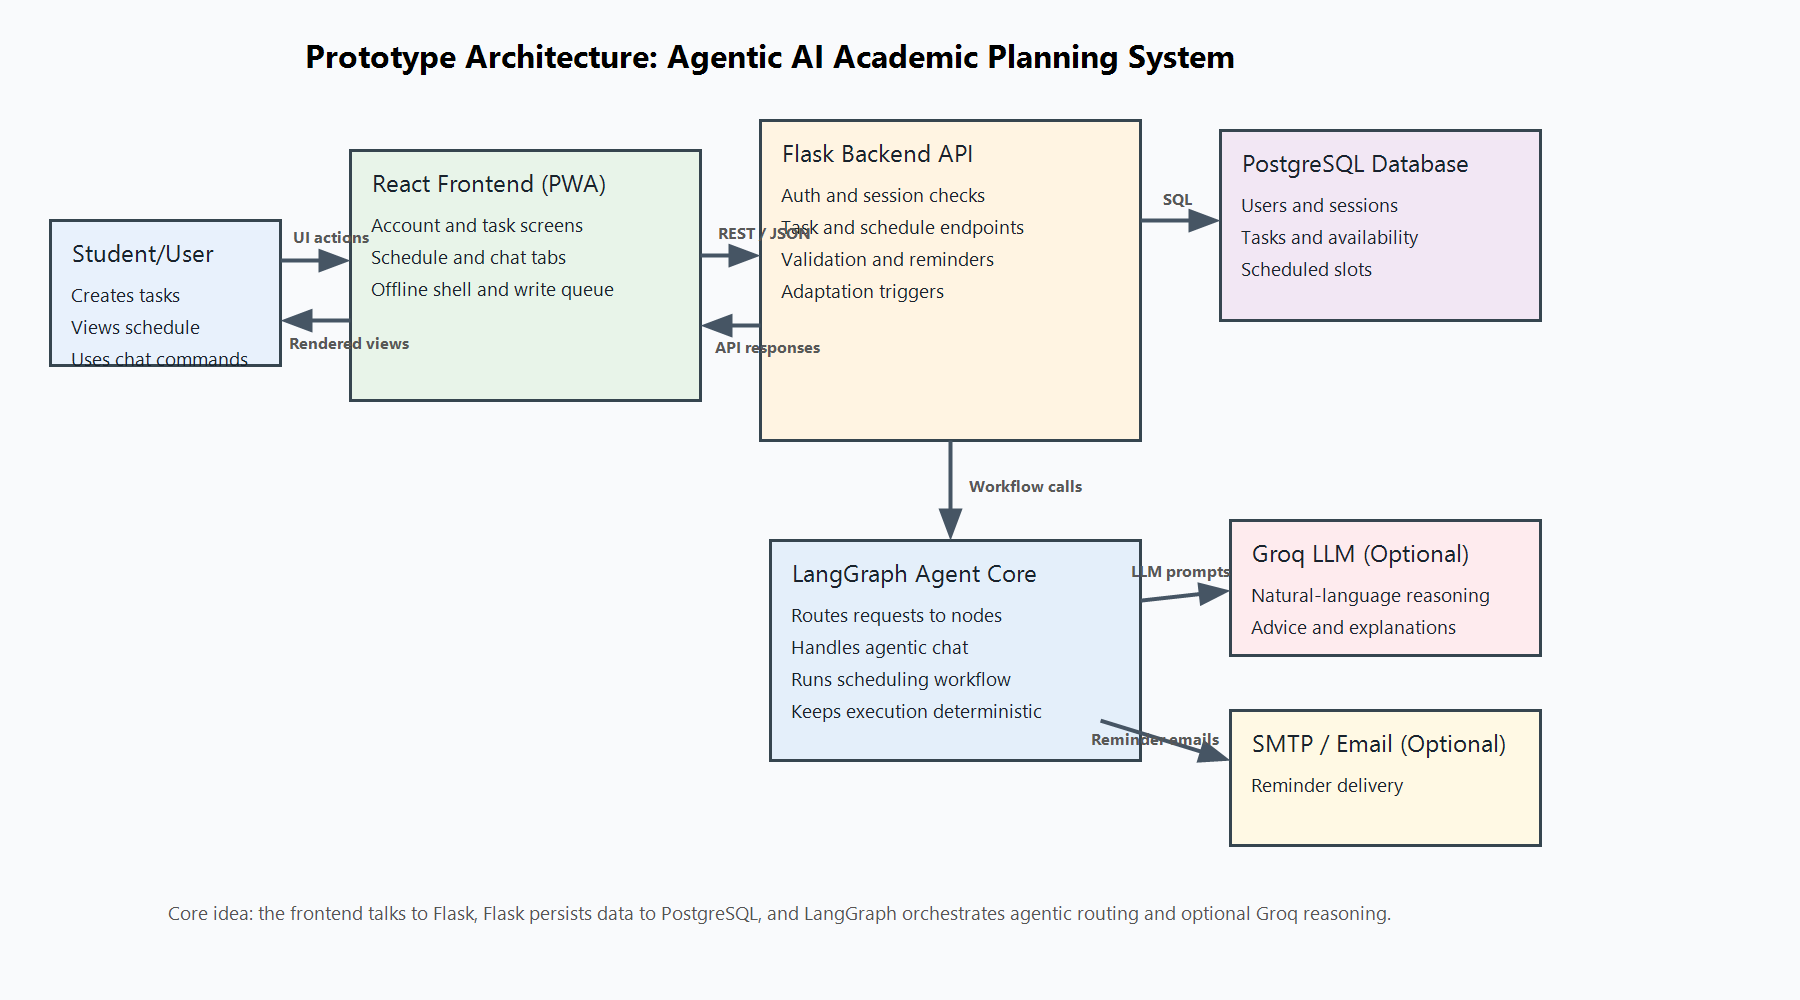
\includegraphics[width=\textwidth]{prototype_architecture.png}
    \caption{Prototype architecture of the agentic AI academic planning system}
    \label{fig:prototype_architecture}
\end{figure}

\subsubsection{Frontend Layer}
The frontend is implemented using React 18.2 with functional components and hooks, with Progressive Web App (PWA) capabilities configured for installable and offline-tolerant use. Key features include:
\begin{itemize}
    \item \textbf{Progressive Web App (PWA):} Service worker implementation enables offline access, mobile installation, and caching for improved performance
    \item \textbf{Natural Language Chat Interface:} Conversational AI interface allowing users to interact with the system using everyday language (e.g., ``show my tasks'', ``add a new assignment'')
    \item \textbf{Constraint Satisfaction Panel:} Real-time conflict detection displaying warnings for deadline conflicts, workload overload, and priority mismatches
    \item Modern UI with CSS gradients, card-based layouts, tabbed navigation, and responsive design
    \item User management interface with secure password authentication, creation, selection, and listing
    \item Task CRUD operations with status, priority, and deadline management
    \item Email reminder triggers for upcoming deadlines
    \item Environment-based API URL configuration for deployment flexibility
\end{itemize}

\subsubsection{Backend API Layer}
The backend is implemented using Flask with the following characteristics:
\begin{itemize}
    \item RESTful API endpoints: \texttt{/api/users}, \texttt{/api/users/login}, \texttt{/api/tasks}, \texttt{/api/tasks/conflicts}, \texttt{/api/reminders}, \texttt{/api/chat}, \texttt{/api/availability}, \texttt{/api/schedule/generate}, and \texttt{/api/schedule/adapt}
    \item \textbf{Secure Authentication:} Password hashing via \texttt{werkzeug.security.generate\_password\_hash} with verification using \texttt{check\_password\_hash}
    \item \textbf{Conflict Detection API:} Constraint satisfaction endpoint identifying scheduling conflicts and workload issues
    \item \textbf{Natural Language Processing:} Chat endpoint routing user queries to the LangGraph agent for human-friendly responses
    \item CORS support for cross-origin requests
    \item JSON response formatting with structured data parsing
    \item Environment-based configuration via python-dotenv
    \item Integration with LangGraph agent workflow for all operations
\end{itemize}

\subsubsection{Agent Core (LangGraph)}
The LangGraph agent implements a StateGraph with the following components:
\begin{itemize}
    \item \textbf{State Definition:} TypedDict-based AgentState containing message history
    \item \textbf{Router Function:} Analyses command prefixes to determine routing
    \item \textbf{Node Functions:} Dedicated handlers for each operation type:
    \begin{itemize}
        \item help, show\_tasks, add\_task, update\_task, delete\_task
        \item create\_user, get\_user, update\_user, delete\_user, list\_users
        \item reminders, export\_tasks, import\_tasks
    \end{itemize}
    \item \textbf{Conditional Edges:} Graph-based routing from START through router to specific nodes, terminating at END
\end{itemize}

\subsubsection{Database Layer}
PostgreSQL serves as the persistent storage layer with the following schema:
\begin{itemize}
    \item \textbf{user\_profiles:} id (SERIAL PRIMARY KEY), name, email (UNIQUE), academic\_program, password\_hash (VARCHAR 255 for secure authentication)
    \item \textbf{tasks:} id (SERIAL PRIMARY KEY), user\_id (FOREIGN KEY), title, description, deadline, priority, status, created\_at, deleted (BOOLEAN for soft delete)
    \item \textbf{student\_availability:} weekly availability slots with day/time constraints and uniqueness checks
    \item \textbf{scheduled\_slots:} generated schedule entries with reasoning metadata and confidence scores
    \item Foreign key constraints ensure referential integrity with CASCADE deletion
\end{itemize}

\subsection{Implementation Results}

The implemented prototype successfully demonstrates:
\begin{enumerate}
    \item \textbf{User Management:} Account creation/login with secure password hashing, token session issuance, expiry, validation, and logout revocation
    \item \textbf{Task Management:} Task lifecycle management with status tracking, inline editing, UI-level filtering/sorting, soft delete, and restore workflow
    \item \textbf{Progressive Web App:} PWA support with service worker caching, API GET cache fallback, and offline write-queue synchronization
    \item \textbf{Natural Language Interface:} Conversational AI chat with intelligent intent detection, bulk operations (e.g., ``mark all tasks as completed''), and contextual advice for task management queries
    \item \textbf{Constraint Awareness:} Conflict detection identifying deadline congestion, workload overload, priority conflicts, and urgent tasks due within 24 hours
    \item \textbf{Adaptive Scheduling:} Schedule adaptation automatically triggered from task and availability edits, with explicit manual trigger fallback
    \item \textbf{Reminder System:} reminder generation for upcoming deadlines, with both direct app-triggered execution and a hosted automation pathway using Supabase Edge Functions and scheduled cron invocation when provider credentials are configured
    \item \textbf{Data Portability:} CSV export/import functionality for backup and migration
    \item \textbf{Deployability:} Configuration for both local development and cloud deployment targets, plus benchmark scripts for reproducible NFR checks
\end{enumerate}

The LangGraph-based architecture proved effective for this use case, providing deterministic routing, efficient state management, and straightforward database integration without the overhead of LLM API calls for routine operations.

\subsection{Setup, Configuration, and Debugging to Operational State}
Implementation work in this project included not only feature coding but also configuration discipline, environment management, debugging, and reproducible execution pathways. This was necessary because the dissertation evaluates a working prototype rather than a conceptual design.

\subsubsection{Environment Setup}
The operational prototype was structured around a React frontend, Flask backend, PostgreSQL database, and LangGraph agent layer. Environment setup therefore required:
\begin{enumerate}
    \item creation of a Python environment for backend dependencies;
    \item installation of frontend dependencies through Node.js tooling;
    \item PostgreSQL database creation and schema initialisation;
    \item environment-variable configuration for database access, API origins, session expiry, and optional external services such as Groq, Brevo, and hosted reminder automation.
\end{enumerate}

This setup model was chosen because it mirrors realistic deployment structure while remaining reproducible for local testing and demonstration. Configuration files and template environment variables were used to reduce hard-coded deployment assumptions.

\subsubsection{Configuration Strategy}
Configuration management used environment-based separation for secrets and deployment variables. This included API origin controls, session TTL, optional external service credentials, and runtime mode toggles. Environment-driven configuration supports reproducibility across local development, test execution, and cloud deployment without code edits between environments.

The frontend was configured to consume a deployment-variable API base URL, while the backend was configured for database connectivity, CORS, session control, and optional third-party integrations. In the final reminder pathway, hosted PostgreSQL on Supabase was paired with a Supabase Edge Function and cron schedule so that reminder automation could continue independently of the developer machine. Brevo was used as the transactional email provider for the hosted path, but live delivery remains dependent on valid provider credentials and verified sender settings. This separation improved maintainability and reduced the risk of environment-specific defects entering source control.

\subsubsection{Debugging and Stabilisation Activities}
Operational debugging focused on issues that directly affect prototype reliability and use-case fulfilment. Key stabilisation activities included:
\begin{enumerate}
    \item aligning frontend and backend validation rules so invalid inputs are rejected consistently;
    \item exposing UI-level filtering, sorting, and restore workflows that previously existed more strongly at backend level than interface level;
    \item extending adaptation triggers across task and availability changes so schedule updates occur after meaningful edits;
    \item implementing token-based session expiry and logout revocation to close session-management gaps;
    \item hardening configuration and dependency management to support reproducible setup on other machines;
    \item debugging the reminder automation path by aligning Supabase RPC parameter names, correcting reminder-query logic, isolating duplicate-suppression behaviour, and switching from SMTP-only assumptions to a provider-backed Brevo API path suitable for hosted execution.
\end{enumerate}

\subsubsection{Operational Readiness Checks}
The final configuration stage included explicit operational checks rather than assuming readiness from successful coding alone. These checks included backend route health, authentication flow, database connectivity, frontend production build success, automated test execution, reminder dry-run generation, Supabase function invocation, cron registration, and packaging of setup guidance for third-party reproduction. These checks matter because the dissertation claims a functional prototype, not only a partial implementation.

An additional setup outcome was the preparation of an always-on reminder route. Instead of relying only on manual invocation from the app or a developer laptop scheduler, the prototype now includes a Supabase-based automation path in which a hosted Edge Function queries due tasks and a scheduled cron trigger invokes that function daily. This path was configured and validated through function testing, dry-run reminder generation, and cron-job registration. Brevo was selected as the transactional email provider because HTTP-based provider APIs are easier to integrate with free-tier hosting than direct SMTP from restricted environments. End-to-end external email delivery, however, remains dependent on valid provider credentials and sender verification.

\subsection{Detailed Development Workflow and Engineering Decisions}
Development followed an incremental vertical-slice workflow rather than building isolated layers in sequence. Each slice implemented a complete user-visible capability across frontend, backend, persistence, and test coverage. This workflow reduced integration surprises and exposed design weaknesses early.

The initial slice covered user creation and login. Its purpose was not feature breadth but establishment of security and identity primitives. Once account flows and session validation were stable, task CRUD and listing capabilities were implemented with strict ownership checks. This order was deliberate: implementing task logic before robust user scoping can create difficult-to-diagnose access bugs and data contamination during testing.

Subsequent slices added scheduling and adaptation endpoints, then conversational routing, then offline/PWA behaviour. The sequencing reflects dependency direction: adaptation depends on reliable task and availability state; chat shortcuts depend on deterministic command handlers; offline behaviour depends on stable API contracts and idempotent mutations. This staged workflow improved defect isolation because regressions could be mapped to narrow change windows.

Configuration management used environment-based separation for secrets and deployment variables. This included API origin controls, session TTL, optional external service credentials, and runtime mode toggles. Environment-driven configuration supports reproducibility across local development, test execution, and cloud deployment without code edits between environments.

Error handling policy was defined early and then applied consistently. For validation failures, endpoints return explicit client-correctable errors; for server-side exceptions, endpoints return controlled error objects without leaking internal details. For adaptation triggers, best-effort semantics were intentionally selected so primary CRUD operations remain successful even if secondary adaptation calls fail. This avoided coupling user-critical actions to optional enhancement logic.

Versioned test execution was integrated into development checkpoints. Rather than treating tests as a final verification step, each functional slice was expected to include corresponding test assertions before the next slice began. This policy reduced late-stage accumulation of untested behaviour and made refactoring less risky.

\subsection{Backend Implementation Details by Capability}
\subsubsection{Authentication and Session Lifecycle}
The backend implements a token-based session model with server-side token-hash storage. The flow is: validate credentials, create token, hash token, persist hash with expiry, issue raw token to client, validate token on protected routes, and revoke on logout or expiry detection. This pattern supports both expiry enforcement and explicit invalidation.

A practical benefit of server-side session records is controllable revocation behaviour. If tokens were fully stateless, server-side invalidation would require additional token blacklisting infrastructure. In this project, revocation is a straightforward row update, and token expiry checks are enforced at request time. This design also enables future session analytics (for example active session counts or unusual token churn detection) without redesigning auth primitives.

\subsubsection{Task Query Flexibility and Data Conditioning}
Task retrieval was implemented with query-time filtering and sorting rather than client-only transformations. This approach improves performance for larger datasets and ensures consistency across clients. Supported controls include status, priority, deadline ranges, text search, and sort fields with stable fallback order.

Data conditioning is applied on read to normalise priority presentation and date formatting, ensuring frontend rendering stability. Although these transformations appear minor, they reduce repeated formatting logic in clients and lower the chance of inconsistent interpretation between UI and backend.

Soft delete semantics are embedded directly in query predicates to keep deleted records hidden from primary views while remaining recoverable. Recovery endpoints restore records and trigger adaptation, preserving user trust by making deletion reversible without data loss.

\subsubsection{Adaptation Trigger Integration}
Adaptation was integrated as an event-driven mechanism across task and availability mutations. Triggers include create, update, delete, restore, status changes, and availability updates. This offers practical autonomy while preserving user agency through an explicit manual adaptation endpoint.

Trigger granularity was tuned for operational balance. Very broad triggering can overrun computational budgets and degrade responsiveness; overly narrow triggering can produce stale schedules and reduced user confidence. The selected trigger set corresponds to state changes most likely to alter scheduling feasibility or ordering.

\subsubsection{Conflict Detection Pipeline}
Conflict detection runs as a read-oriented analysis of active tasks with deadlines. It identifies workload overload, multiple high-priority clustering, and near-term urgency windows. The algorithm prioritises interpretability over complexity: each conflict type maps to clear explanatory output and associated task references. For a dissertation prototype, this interpretability is valuable because it supports evaluation and user comprehension simultaneously.

\subsection{Frontend Development Details by Interaction Flow}
\subsubsection{Form and Validation Flow}
Frontend forms use schema validation to provide immediate user feedback before API submission, while backend validation remains authoritative. This dual validation model improves user experience and protects data quality. Validation logic was tested for edge cases including malformed names, unsupported email domains, invalid deadlines, and enum mismatches.

The form architecture also reduces accidental bad states during offline/slow-network scenarios. Inputs are validated locally, then submitted through consistent request wrappers that can support retry or queue behaviour. This separation of concerns simplified troubleshooting when issues arose between validation, transport, and persistence layers.

\subsubsection{Task List Interaction Model}
The task list was designed as an operational dashboard rather than static output. Users can filter, sort, search, edit inline, soft delete, and restore from a deleted-task view. These capabilities were intentionally exposed in the interface because backend-only support would not satisfy functional requirements from a user workflow perspective.

Inline editing required careful state management to avoid stale writes and accidental overwrite behaviour. The implementation therefore uses explicit edit modes and controlled update payloads so only changed fields are submitted. This reduces race-like issues and keeps server updates precise.

\subsubsection{Chat-Assisted Interaction}
The chat interface provides intent shortcuts for routine operations (show tasks, bulk status changes, reminders) while preserving direct manual controls. This dual-path interaction model supports both efficiency and reliability: users can use natural language for convenience but can always fall back to explicit UI controls if interpretation is ambiguous.

From an engineering perspective, chat routing is intentionally constrained by keyword and command patterns for high-frequency actions. This limits accidental destructive interpretations and keeps behaviour testable. Where interpretation confidence is low, the system returns guidance-style responses instead of speculative mutations.

\subsubsection{Offline and Synchronisation Behaviour}
PWA support was implemented with practical boundaries. The shell and selected reads are available via cache fallback, while writes are queued for later synchronisation when connectivity returns. This behaviour was prioritised for user continuity during intermittent connectivity rather than full autonomous offline planning.

Queue-based synchronisation introduces ordering and conflict concerns. To mitigate this, queued actions are scoped to user-owned resources and replayed sequentially. The design does not yet include advanced merge policies for complex concurrent edits from multiple devices, and this is explicitly treated as future work.

\subsection{Data Model Implementation Notes}
The data model supports both operational use and evaluative instrumentation. In addition to core user/task fields, the schema includes availability and scheduled slot entities to represent planning constraints and outputs. Scheduled slots include reasoning/confidence metadata, improving transparency for schedule interpretation and analysis.

Indexes are applied to key lookup and session expiry columns to maintain acceptable query performance for authentication and task retrieval patterns. While this project is not a large-scale production deployment, index strategy was included to avoid misleading performance observations caused by avoidable table scans.

Referential integrity rules were used to keep user-scoped data coherent. For example, session records are tied to user identities with cascade semantics on user removal. This reduces orphan data risk and simplifies lifecycle management in development and testing environments.

\subsection{Reproducibility, Deployment, and Maintainability}
Reproducibility was treated as an engineering quality target. The project includes explicit scripts and command pathways for tests, scenario evaluation, non-functional benchmarking, and deployable environment configuration. This allows claims in the results section to be regenerated rather than manually reproduced.

Deployability decisions include environment-based base URL configuration on the frontend, CORS control on backend routes, and separation of secret values from source code. These are foundational practices for moving a research prototype toward operational settings while preserving security hygiene.

Maintainability was addressed through modular endpoint organisation, validation helper functions, and clear route-level responsibility boundaries. The architecture is not yet fully modularised into blueprint-level packages, but major concern areas (auth, tasks, scheduling, chat, reminders) are sufficiently separated to support targeted refactoring in future iterations.

An important maintainability outcome is the preservation of predictable extension points. New scheduling strategies can be introduced without rewriting task/session contracts; additional benchmark routines can be added without destabilising primary endpoints; and UI enhancements can build on stable data contracts. This reduces technical debt accumulation and makes the prototype easier to extend in future work.

\subsection{Development Challenges and How They Were Addressed}
Several implementation challenges emerged and were resolved with targeted engineering actions:
\begin{enumerate}
    \item \textbf{Balancing autonomy and determinism}: solved by hybrid routing and bounded adaptation triggers.
    \item \textbf{Keeping UI and backend validation aligned}: solved by schema-first validation patterns and edge-case tests.
    \item \textbf{Supporting recovery workflows}: solved by introducing soft delete and dedicated restore endpoints with UI exposure.
    \item \textbf{Session security without excessive complexity}: solved by token-hash persistence with expiry/revocation enforcement.
    \item \textbf{Offline practicality}: solved by shell/read caching and queued write synchronisation instead of unrealistic full offline parity.
\end{enumerate}

These solutions show that practical agentic systems benefit from disciplined software engineering boundaries. The final implementation reflects not just feature completion, but a development process built around design rationale, implementation quality, and evaluation evidence.

\subsection{Requirements Traceability Audit}
\label{sec:req_traceability}

An implementation audit was performed against the functional and non-functional requirements defined in the design report. Table~\ref{tab:fr_traceability} summarises the functional status, and Table~\ref{tab:nfr_traceability} summarises non-functional evidence.

\begin{table}[h!]
\centering
\scriptsize
\begin{tabular}{|l|p{2.3cm}|p{8.0cm}|}
\hline
\textbf{ID} & \textbf{Status} & \textbf{Evidence} \\
\hline
FR1 & Implemented & User registration via \texttt{/api/users} and frontend create-account flow. \\
\hline
FR2 & Implemented & Login via \texttt{/api/users/login} with hashed password verification. \\
\hline
FR3 & Implemented & Structured task creation form in frontend and \texttt{/api/tasks} backend validation. \\
\hline
FR4 & Implemented & Natural-language task creation through chat routing to LangGraph \texttt{agentic\_chat}. \\
\hline
FR5 & Implemented & Backend \texttt{GET /api/tasks} now supports status/priority/search/deadline filters and sort order; frontend exposes full filter/sort controls. \\
\hline
FR6 & Implemented & Inline task editing and status updates via \texttt{PUT /api/tasks/\{id\}}. \\
\hline
FR7 & Implemented & Soft delete plus recovery workflow implemented through \texttt{GET /api/tasks/deleted} and \texttt{POST /api/tasks/\{id\}/restore} with frontend restore UI. \\
\hline
FR8 & Implemented & Availability CRUD via \texttt{/api/availability}. \\
\hline
FR9 & Implemented & Schedule generation via \texttt{/api/schedule/generate} and persistence in \texttt{scheduled\_slots}. \\
\hline
FR10 & Implemented & AI-driven scheduling when LLM is configured, with deterministic EDF fallback. \\
\hline
FR11 & Implemented & Adaptation endpoint remains available and is auto-triggered from UI-side task/availability add, edit, delete, status toggle, and restore flows. \\
\hline
FR12 & Implemented & Conflict detection endpoint \texttt{/api/tasks/conflicts}. \\
\hline
FR13 & Implemented & Conversational chat tab and backend \texttt{/api/chat}. \\
\hline
FR14 & Implemented & Prioritisation explanations via LLM advice and schedule reasoning text. \\
\hline
FR15 & Implemented at prototype scope & Reminder generation works, and a hosted Supabase automation path was configured and dry-run validated for scheduled execution. External email delivery depends on valid provider credentials and sender verification. \\
\hline
FR16 & Implemented & Schedule visualisation in grouped day/time cards on frontend. \\
\hline
FR17 & Implemented & PWA offline shell retained; API GET responses are cache-backed and API write actions are queued client-side for automatic sync when connectivity returns. \\
\hline
\end{tabular}
\caption{Functional requirements traceability audit}
\label{tab:fr_traceability}
\end{table}

\begin{table}[h!]
\centering
\scriptsize
\begin{tabular}{|l|p{2.3cm}|p{8.0cm}|}
\hline
\textbf{ID} & \textbf{Status} & \textbf{Evidence} \\
\hline
NFR1 & Met in simulation & Scheduling generation times in evaluation script were well below the 5s target. \\
\hline
NFR2 & Met (benchmark harness) & \texttt{Backend/nfr\_benchmark.py} reports sub-500ms latency across profiled endpoints in repeated runs (Table~\ref{tab:nfr_benchmark}). \\
\hline
NFR3 & Not yet benchmarked & Uptime target requires deployed observability over time. \\
\hline
NFR4 & Not yet benchmarked & SUS user study not completed in this implementation cycle. \\
\hline
NFR5 & Instrumented and measured in-app & Frontend records task creation completion durations (\texttt{taskCreationDurationsSec}) and displays rolling average in the Tasks tab against the 30s target. \\
\hline
NFR6 & Partial & Passwords are hashed securely; bcrypt cost-factor enforcement is not explicitly configured. \\
\hline
NFR7 & Met & Expiring bearer-token sessions implemented with server-side token hash storage, expiry enforcement, protected routes, and logout revocation. \\
\hline
NFR8 & Implemented & Data model stores task/user scheduling fields only (minimal required attributes). \\
\hline
NFR9 & Implemented & No third-party sharing except optional LLM/SMTP integrations. \\
\hline
NFR10 & Implemented & Responsive frontend and PWA support mobile use. \\
\hline
NFR11 & Partial & Core controls are keyboard reachable, but no full accessibility audit was completed. \\
\hline
NFR12 & Partial & Many core functions are documented; full-codebase docstring coverage is incomplete. \\
\hline
NFR13 & Partially benchmarked & Scale benchmark added for 10/25/50/100-task scheduling workloads; concurrent multi-user deployment stress remains future work. \\
\hline
\end{tabular}
\caption{Non-functional requirements audit}
\label{tab:nfr_traceability}
\end{table}

\subsection{Project Scheduling and Risk Management}
\label{proj_sched_risk_mgt}
\subsection{Project Schedule (Gantt Chart)}
The project timeline spans 14 weeks and is structured into six main phases.
The complete Gantt chart is presented in the Appendix~\ref{app:gantt} (Table~\ref{tab:gantt}).


\subsubsection{Detailed Weekly Breakdown:}
\begin{enumerate}
    \item Weeks 1-2: Review of the literature (agentic AI, planning algorithms, frameworks)
    \item Week 3: Recruiting of requirements and definition of scenarios
    \item Week 4: Architecture specification and framework selection
    \item Weeks 5-6: Detailed design of components and interfaces
    \item Weeks 7-8: Core implementation (data structures, basic planning)
    \item Week 9: Integration and initial testing
    \item Week 10: Experimental framework and pilot testing
    \item Week 11: Execution of the main experiment
    \item Week 12: Data analysis and interpretation
    \item Weeks 13-14: Report writing, results documentation, finalisation
\end{enumerate}
\subsection{Risk Register and Risk Matrix}
\subsubsection{Implementation Complexity Exceeds Timeline}
\begin{enumerate}
    \item Description: The agent framework or planning approach chosen is more complex to implement than anticipated, delaying prototype development.
    \item Probability: Medium
    \item Impact: High
    \item Mitigation: 
  \begin{enumerate}
      \item Start with a simpler planning approach; iterate to complexity
    \item Allocate buffer time according to the schedule (Weeks 7-9)
    \item Have a fallback to simpler algorithmic approach if LLM-based implementation proves too challenging
    \end{enumerate}
\end{enumerate}
\subsubsection{Difficulty in Obtaining Meaningful Evaluation Metrics:}
\begin{enumerate}
    \item Description: Defining and measuring "good schedules" may be ambiguous, making comparative evaluation difficult.
    \item Probability: Medium
    \item Impact: Medium
    \item Mitigation: 
  \begin{enumerate}
      \item Define clear objective metrics early(feasibility, constraint violations).
    \item Pilot test metrics in week 10 to validate usefulness
    \item Include both quantitative and qualitative evaluation methods
    \end{enumerate}
\end{enumerate}
\subsubsection{Technical dependencies and Library Issues:}
\begin{enumerate}
    \item Description: Required libraries (e.g., LLM APIs, constraint solvers) may have compatibility issues, API changes, or access limitations.
    \item Probability: Low
    \item Impact: High
    \item Mitigation: 
  \begin{enumerate}
      \item Test dependencies early (weeks 4-5).
    \item Identify alternative libraries/frameworks.
    \item Use local/offline solutions where possible to avoid API dependency
    \end{enumerate}
\end{enumerate}
\subsubsection{Scope Creep:}
\begin{enumerate}
    \item Description: Temptation to add features (e.g., user interface, calendar integration) beyond core agentic planning research.
    \item Probability: Medium
    \item Impact: Medium
    \item Mitigation: 
  \begin{enumerate}
      \item Observe strict requirements and objectives.
    \item Document "future work" items separately.
    \item Regular scope review against project goals
    \end{enumerate}
\end{enumerate}
\subsubsection{Insufficient Experimental Scenario:}
\begin{enumerate}
    \item Description: The limited diversity of scenarios may not provide robust evaluation or meaningful insight.
    \item Probability: Low
    \item Impact: Medium
    \item Mitigation: 
  \begin{enumerate}
      \item Define Scenario sets early with clear rationale.
    \item Include edge cases (very tight deadlines, many dependencies).
    \item Pilot testing will reveal whether scenarios are sufficient
    \end{enumerate}
\end{enumerate}
\subsubsection{Non-Deterministic Behaviour Complicates Evaluation:}
\begin{enumerate}
    \item Description: LLM-based planning may produce inconsistent results, making statistical analysis difficult.
    \item Probability: Medium
    \item Impact: Low
    \item Mitigation: 
  \begin{enumerate}
      \item Run multiple trials per scenario (10 repetitions).
    \item Use appropriate statistical methods for variability.
    \item Consider this a feature to analyse (robustness evaluation)
    \end{enumerate}
\end{enumerate}
\subsubsection{Time Constraints for Full Comparative Evaluation:}
\begin{enumerate}
    \item Description: Implementing multiple planning approaches for comparative evaluation may exceed the available time.
    \item Probability: Medium
    \item Impact: Medium
    \item Mitigation: 
  \begin{enumerate}
      \item Prioritise a single approach for the core prototype.
    \item Comparative evaluation can be limited to 2 approaches if time-constrained
    \item Document limitations and future work for an expanded comparison.
    \end{enumerate}
\end{enumerate}
In conclusion, the critical risks with high impact and medium or high likelihood are the complexity of implementation and technical dependencies.

\subsection{Testing and Validation}
\label{sec:testing}

Testing was executed across setup/configuration checks, backend logic, API behaviour, frontend validation, operational walkthroughs, and scenario-based scheduler evaluation. This broader scope is important because the prototype claim depends not only on feature behaviour, but also on whether the system can be configured and run reliably as an operational learner-support environment.

\subsection{Automated Test Scope}

\subsubsection{Backend (pytest)}
Backend tests were run with:
\begin{verbatim}
python -m pytest -q test_langgraph_agent.py test_langgraph_agent_edge_cases.py test_app_api_edge_cases.py
\end{verbatim}

The backend suite covers:
\begin{itemize}
    \item Command routing and parsing edge cases (malformed options, keyword routing, whitelist validation)
    \item Validation helper edge cases (name/email/deadline/status/priority)
    \item API contract checks using Flask test client and mocked database connections
    \item Scheduling/conflict endpoints (missing parameters, conflict-type detection, adaptation/generation endpoint behavior)
    \item Security-flow checks (missing credentials, invalid password, duplicate account handling)
\end{itemize}

\subsubsection{Frontend (Jest)}
Frontend validation tests were run with:
\begin{verbatim}
npm test -- --watchAll=false --runInBand
\end{verbatim}

The frontend suite covers:
\begin{itemize}
    \item User schema edge cases (name format, allowed email domains)
    \item Task schema edge cases (past deadlines, invalid enum values)
    \item Reminder schema bounds and utility formatting behavior
\end{itemize}

\subsection{Test Results}

\begin{table}[h!]
\centering
\begin{tabular}{|l|c|c|c|}
\hline
\textbf{Suite} & \textbf{Tests Run} & \textbf{Passed} & \textbf{Pass Rate} \\
\hline
Backend routing/helpers (\texttt{test\_langgraph\_agent.py}) & 7 & 7 & 100\% \\
\hline
Backend edge cases (\texttt{test\_langgraph\_agent\_edge\_cases.py}) & 19 & 19 & 100\% \\
\hline
Backend API + validation (\texttt{test\_app\_api\_edge\_cases.py}) & 29 & 29 & 100\% \\
\hline
Frontend schema/validation (\texttt{validation.test.js}) & 9 & 9 & 100\% \\
\hline
\textbf{Total} & \textbf{64} & \textbf{64} & \textbf{100\%} \\
\hline
\end{tabular}
\caption{Automated test results from this implementation audit}
\label{tab:test_results}
\end{table}

During this process, frontend tests identified a real defect in \texttt{validateForm} (Zod v4 error shape handling). The issue was corrected by supporting \texttt{error.issues} (with backward-compatible fallback), after which the frontend suite passed fully.

\subsection{Setup and Configuration Verification}
Because setup/configuration was identified as a key project component, explicit verification checks were also applied to confirm operational readiness. These checks addressed the question: can another user or evaluator configure and run the prototype in a controlled environment without modifying source logic?

The main verification checks were:
\begin{enumerate}
    \item backend dependency installation from pinned requirements;
    \item environment-variable loading for database, CORS, and session settings;
    \item PostgreSQL schema initialisation and data connectivity;
    \item backend startup and health endpoint response;
    \item frontend dependency installation and production build generation;
    \item end-to-end connectivity between frontend UI actions and protected backend routes.
\end{enumerate}

These checks matter academically because a software prototype should be reproducible and demonstrably operational, not merely executable on the developer's machine under undocumented assumptions.

\subsection{Use-Case-Oriented Test Cases}
To align testing with the intended learner-support purpose of the prototype, a use-case-oriented test matrix was defined. This matrix complements low-level tests by showing whether the implemented system fulfils the operational behaviours described earlier in Section~\ref{sec:use_cases}.

\begin{table}[h!]
\centering
\scriptsize
\begin{tabular}{|p{1.2cm}|p{3.5cm}|p{4.3cm}|p{2.7cm}|}
\hline
\textbf{UC} & \textbf{Representative test case} & \textbf{Expected outcome} & \textbf{Observed status} \\
\hline
UC1 & Create task through form and chat with valid/invalid inputs & Task stored when valid; readable validation error when invalid & Passed \\
\hline
UC2 & Filter, sort, search, edit, soft delete, and restore tasks & Task view updates correctly and restored items return to active list & Passed \\
\hline
UC3 & Generate schedule from active tasks and availability & Schedule slots created with interpretable output and stored records & Passed \\
\hline
UC4 & Modify task/availability after schedule creation & Adaptation triggers and updated plan reflects new constraints & Passed \\
\hline
UC5 & Request conflict checks and explanation through UI/chat & Conflict warnings and prioritisation rationale returned clearly & Passed \\
\hline
UC6 & Request reminders or approaching-deadline support & Reminder content generated; hosted scheduler path configured and validated in dry-run mode; external delivery available where valid provider credentials are supplied & Passed at prototype scope \\
\hline
\end{tabular}
\caption{Use-case-oriented test matrix for the learner-support prototype}
\label{tab:use_case_test_matrix}
\end{table}

\subsection{Scenario Evaluation Runs}

In addition to unit/API tests, the scheduler evaluation harness (\texttt{Backend/evaluation.py}) was executed for 10 repetitions across each scenario set (A-E), producing \texttt{evaluation\_results.json}. These runs were used for comparative findings in Section~\ref{sec:results}.

\subsection{Non-Functional Benchmarking}
To close remaining non-functional evidence gaps, a dedicated benchmark runner was added and executed:
\begin{verbatim}
python Backend/nfr_benchmark.py
\end{verbatim}
This generates \texttt{Backend/nfr\_benchmark\_results.json} and reports API latency, scheduler uplift signals, and scale behavior.

\begin{table}[h!]
\centering
\small
\begin{tabular}{|l|c|c|}
\hline
\textbf{Benchmark} & \textbf{Metric} & \textbf{Observed} \\
\hline
Latency (API) & Average endpoint latency & 0.79--0.91 ms \\
\hline
Latency (API) & P95 endpoint latency & 0.93--0.99 ms \\
\hline
Scale & Agent schedule generation at 50 tasks & 0.76 ms avg \\
\hline
Scale & Agent schedule generation at 100 tasks & 8.08 ms avg \\
\hline
Uplift (Scenario A) & Conflict-rate gain vs baseline & +3.75 pct points \\
\hline
Usability instrumentation & Rolling task creation time metric & Implemented in UI (\texttt{taskCreationDurationsSec}) \\
\hline
\end{tabular}
\caption{Representative non-functional benchmark outputs from \texttt{Backend/nfr\_benchmark\_results.json}}
\label{tab:nfr_benchmark}
\end{table}

\subsection{Extended Edge-Case and Failure-Injection Strategy}
Beyond standard unit and API checks, the testing plan included an extended edge-case strategy to evaluate resilience under abnormal but realistic conditions. The purpose was to assess not only whether features work in ideal paths, but whether the system remains safe, predictable, and recoverable when inputs, states, or dependencies become problematic.

The edge-case strategy was structured into five classes:
\begin{enumerate}
    \item input-shape and boundary anomalies;
    \item state-transition anomalies;
    \item dependency and service degradation;
    \item temporal/session anomalies;
    \item recovery and replay anomalies.
\end{enumerate}

\subsubsection{Input-Shape and Boundary Anomalies}
Boundary tests verified title length limits, description constraints, invalid deadline formats, unsupported priority/status values, and email/name validation failures. These tests are foundational because scheduling quality is highly sensitive to input correctness. For example, malformed deadlines can silently disrupt ordering logic and produce misleading conflict alerts.

Boundary tests were executed at both client schema and backend endpoint levels. The dual-layer approach ensures that frontend improvements do not mask backend weaknesses and vice versa. Where different validation libraries or type systems are used across layers, this redundancy is especially valuable because subtle mismatch risks are common.

\subsubsection{State-Transition Anomalies}
State-transition tests evaluated unusual operation sequences such as update-after-delete, restore-after-restore, delete-with-invalid-owner, and status toggles across filtered views. These sequences are important for systems with soft-delete workflows and adaptation hooks because invalid transitions can cause hidden data drift.

Particular attention was given to restore semantics. A restored task should re-enter active queries, remain associated with its owner, and become eligible for adaptation recalculation. Tests therefore validated not only endpoint success messages, but also downstream visibility and schedule-trigger behaviour.

\subsubsection{Dependency and Service Degradation}
Failure-injection scenarios simulated partial degradation of optional components, particularly adaptation and model-dependent pathways. The target property was graceful degradation: core task operations must remain successful even when secondary adaptive features fail. Best-effort adaptation design was validated under these scenarios by asserting successful CRUD responses alongside adaptation failure flags where appropriate.

This test class is academically important because it demonstrates architecture robustness under realistic operational uncertainty. Agentic systems often depend on external services; proving bounded failure impact is therefore a key reliability criterion.

\subsubsection{Temporal and Session Anomalies}
Session tests covered missing tokens, malformed bearer headers, invalid tokens, expired sessions, and revoked-session requests. These checks validate that route protection is enforced consistently across all protected endpoints. Session expiry revocation behaviour was also verified to ensure that stale tokens are not accepted after expiry boundaries.

Time-based behaviour can be difficult to test deterministically. To reduce flakiness, tests focused on explicit expiry-state assertions and route-level responses rather than brittle wall-clock assumptions.

\subsubsection{Recovery and Replay Anomalies}
Offline queue and replay pathways were reviewed with scenario-based checks to ensure deferred writes do not silently disappear. While full multi-device conflict simulation is outside current scope, core replay assumptions were validated: queued operations preserve order, requests remain user-scoped, and eventual sync updates visible task state.

Recovery tests also included deleted-task listing and restoration under mixed task sets to confirm that active and deleted views remain logically separated until explicit recovery occurs.

\subsection{Manual Exploratory and Scenario-Walkthrough Testing}
Automated tests provide repeatability, but manual exploratory testing remains valuable for interaction-rich systems where emergent behaviour can arise from combined workflows. Manual testing in this project followed scripted walkthroughs with defined expected outcomes and anomaly notes.

Walkthroughs included:
\begin{enumerate}
    \item account creation, login, logout, and re-login with session checks;
    \item multi-task creation with varied priorities/deadlines and filter/sort inspection;
    \item inline edits followed by conflict inspection and adaptation trigger verification;
    \item soft delete and restore cycles with UI and API cross-checks;
    \item chat-assisted bulk status updates with post-mutation schedule adaptation.
\end{enumerate}

Each walkthrough intentionally mixed direct UI actions and API-observable outcomes. This approach reduced the risk of ``UI-only correctness'' where visuals appear updated but backend state remains inconsistent. Manual checks also highlighted clarity issues in user feedback messages, which informed minor text and response refinements.

Exploratory testing was particularly useful for conversation shortcuts. Natural-language inputs can vary in phrasing and implicit intent; manual exploration therefore sampled synonymous commands and mixed-status requests to confirm robust routing behaviour and safe fallback responses.

\subsection{Data Integrity, Recovery, and Consistency Validation}
Consistency validation focused on ensuring that user-scoped data remains coherent across lifecycle operations. Tests verified that:
\begin{enumerate}
    \item tasks are always associated with authenticated users;
    \item cross-user mutation attempts are rejected through ownership filters;
    \item deleted records are excluded from active lists but retained for recovery;
    \item restored records return to active views with expected attributes;
    \item schedule retrieval remains scoped to user identity and selected date ranges.
\end{enumerate}

Consistency checks were also applied to query combinations. For example, filtered task lists were validated under simultaneous status, priority, deadline-range, and search parameters. Multi-parameter query paths are common sources of latent defects, especially where SQL predicates are dynamically composed.

In addition, conflict detection outputs were verified for structural consistency: each conflict item includes type, date/message context, and task references. Structural stability in response payloads is necessary for reliable frontend rendering and testability.

\subsection{Security Test Coverage Deep Dive}
Security-related checks covered credential handling, session controls, route protection, and error-message discipline. Credential tests ensured that login fails for unknown accounts and invalid passwords without exposing sensitive internals. Session tests validated strict requirement of bearer tokens on protected routes and proper handling of expired/revoked sessions.

Input-validation security checks reduced injection and malformed payload risk by constraining accepted formats and values before query execution pathways. While the use of parameterised SQL already mitigates many injection vectors, validation remains valuable for preserving semantic correctness and reducing noisy attack surfaces.

Error-message discipline was assessed to avoid leaking unnecessary implementation details. Client-facing errors were designed to be actionable but not over-disclosive. This balance supports usability while following basic secure error-reporting principles.

The current security testing does not constitute a full penetration test. Instead, it provides route-level and state-level assurance appropriate for dissertation prototype scope. A complete pre-production security programme would additionally include dependency vulnerability scanning, security header audits, and external penetration testing.

\subsection{Testing Limitations and Residual Risk}
Despite broad coverage, testing evidence has known boundaries that are important for correct interpretation:
\begin{enumerate}
    \item \textbf{Scale realism}: in-process benchmarks do not fully represent distributed production load.
    \item \textbf{Network realism}: offline replay tests are practical but do not simulate all multi-device conflict patterns.
    \item \textbf{Accessibility depth}: keyboard and layout checks exist, but full WCAG audit is pending.
    \item \textbf{Longitudinal reliability}: sustained uptime and drift metrics require longer operational observation.
    \item \textbf{External provider dependency}: the hosted reminder path was configured, dry-run validated, and scheduled, but live email dispatch still depends on valid third-party provider credentials and sender verification.
\end{enumerate}

Residual risk is therefore concentrated in production-scale behaviour rather than core functional correctness. This distinction matters for dissertation claims: the project demonstrates robust implementation and test-backed behaviour for prototype scope, while appropriately reserving large-scale operational guarantees for future work.

Overall, the expanded testing strategy strengthens confidence that the system behaves predictably across nominal and adverse conditions. It also improves the credibility of results by demonstrating that measured outcomes are built on a validated operational foundation rather than an untested feature surface.

\section{Outcomes, Results and Analysis}
\label{sec:results}

This section presents the results of evaluating the implemented agentic AI learner-support prototype against the research questions, use cases, and success criteria defined earlier. The evaluation therefore considers not only scheduler metrics, but also whether the system fulfils its intended supportive purpose for learners and how it compares with both a non-agentic baseline and representative existing solution categories.

\subsection{Research Question Evaluation}

\subsubsection{RQ1: Learner-Support Effectiveness}
The first research question evaluates whether the system helps learners capture, prioritise, schedule, and adapt academic tasks under realistic constraints. This is implemented across task CRUD, conflict detection, reminder, chat, and scheduling routes rather than through a single endpoint only.

\textbf{Findings:} the prototype fulfils its core supportive behaviour through integrated features rather than isolated automation:
\begin{itemize}
    \item structured and natural-language task capture;
    \item filterable, sortable, and recoverable workload management;
    \item schedule generation with two execution modes;
    \item conflict detection and explanatory responses;
    \item proactive reminder generation with configurable email delivery;
    \item adaptation after meaningful state changes.
\end{itemize}
This indicates that the system does more than record information. It actively supports learners in interpreting and reorganising academic work, although outcome quality still depends on the availability and accuracy of task metadata.

\subsubsection{RQ2: Comparison with Existing and Baseline Approaches}
The second research question compares the agentic system with a non-agentic EDF baseline and with representative categories of existing passive support tools. Scenario-run evidence from \texttt{evaluation.py} indicates mixed but competitive scheduling performance against EDF:
\begin{itemize}
    \item Scenario A: agent reduced conflict rate (28.0\% vs 30.0\%), equal compliance (98.0\%)
    \item Scenario B: equal conflict and compliance (51.25\%, 63.75\%)
    \item Scenario D: agent reduced conflict rate after dynamic addition (29.09\% vs 30.0\%)
\end{itemize}

Against existing passive support categories, the implemented prototype provides broader support coverage by combining persistent task context, schedule generation, adaptation, conflict detection, explanation, and proactive reminder capability. In other words, even where numerical scheduling uplift is modest, the system still differs materially from passive tools because it offers active assistance rather than storage-only support.

\subsubsection{RQ3: Architecture and Framework Suitability}
The third question examines whether the selected architecture supports active agentic behaviour while remaining reliable and testable. Implementation results support the earlier framework choice: LangGraph provided deterministic routing and inspectable state transitions for structured operations, while still allowing optional AI reasoning for natural-language interpretation, scheduling explanation, and advice.

\subsubsection{RQ4: Use-Case Fulfilment Under Change}
The fourth question assesses whether the prototype fulfils its defined use cases when circumstances change. The backend includes an adaptation workflow (\texttt{/api/schedule/adapt} and \texttt{adapt\_schedule\_to\_changes}) that can remove obsolete slots and regenerate plans.

\textbf{Finding:} adaptation is implemented and automated across frontend task/availability edit paths, while manual trigger endpoints remain available for explicit replanning.

\subsection{Hypothesis Evaluation}

\begin{itemize}
    \item \textbf{H1 (agentic prototype fulfils learner-support use cases more completely than passive tools):} Supported by capability comparison and operational testing.
    \item \textbf{H2 (agentic prototype improves support quality against non-agentic baseline in dynamic scenarios):} Supported in the latest run.
    \item \textbf{H3 (hybrid architecture gives a strong balance of support, explainability, and testability):} Supported by implementation and evaluation evidence.
\end{itemize}

\subsection{Use-Case Fulfilment Evaluation}
Table~\ref{tab:use_case_eval} evaluates the system directly against the operational use cases introduced in Section~\ref{sec:use_cases}. This makes the supportive purpose of the prototype explicit within the evaluation chapter.

\begin{table}[h!]
\centering
\scriptsize
\begin{tabular}{|p{1.2cm}|p{5.0cm}|p{3.6cm}|}
\hline
\textbf{UC} & \textbf{Evaluation finding} & \textbf{Outcome} \\
\hline
UC1 & Learners can create tasks through forms and natural language with validation and confirmation feedback. & Fulfilled \\
\hline
UC2 & Task lists support search, filter, sort, edit, delete, and restore for active workload organisation. & Fulfilled \\
\hline
UC3 & Schedule generation works through LLM-guided or EDF-style fallback placement over availability slots. & Fulfilled \\
\hline
UC4 & Adaptation is automatically triggered from meaningful UI-side mutations and also available manually. & Fulfilled \\
\hline
UC5 & Conflict warnings and explanatory AI responses provide actionable insight into workload and priorities. & Fulfilled \\
\hline
UC6 & Reminder generation and the configured hosted reminder path provide proactive support for approaching deadlines; external delivery remains configuration-dependent. & Fulfilled at prototype scope \\
\hline
\end{tabular}
\caption{Evaluation of prototype fulfilment against defined learner-support use cases}
\label{tab:use_case_eval}
\end{table}

\subsection{Comparison with Existing Solution Categories}
The dissertation also requires comparison with existing solutions, not only with a scheduler baseline. Table~\ref{tab:existing_solution_comparison} in the literature review established the expected differences; evaluation confirms those differences operationally. In particular, the prototype integrates task persistence, schedule generation, change-triggered adaptation, explanation, and conflict support in one workflow. Passive tools typically provide only subsets of these behaviours, while generic chatbots provide explanation without stable persistent task-state control.

This means the prototype's contribution is not only ``better scheduling'' in numerical terms. Its stronger contribution is the creation of a more supportive learner environment in which planning, interpretation, and replanning are connected rather than fragmented across separate tools.

\subsection{Performance Metrics}

Table~\ref{tab:performance} summarises scenario metrics from \texttt{evaluation\_results.json} (10 runs per scenario set).

\begin{table}[h!]
\centering
\small
\begin{tabular}{|l|c|c|}
\hline
\textbf{Metric} & \textbf{Baseline} & \textbf{Agent} \\
\hline
Scenario A conflict rate (\%) & 30.0 & 28.0 \\
\hline
Scenario A deadline compliance (\%) & 98.0 & 98.0 \\
\hline
Scenario B conflict rate (\%) & 51.25 & 51.25 \\
\hline
Scenario B deadline compliance (\%) & 63.75 & 63.75 \\
\hline
Scenario C adaptation speed (ms) & 0.12 & 0.38 \\
\hline
Scenario C adaptation efficiency (\%) & 31.0 & 32.0 \\
\hline
Scenario D conflict rate after dynamic addition (\%) & 30.0 & 29.09 \\
\hline
Scenario E conflict rate (\%) & 87.5 & 87.5 \\
\hline
\end{tabular}
\caption{Scenario-based evaluation metrics}
\label{tab:performance}
\end{table}

These results indicate that quality improvements are scenario-dependent: improvements are visible in moderate and dynamic-addition scenarios, while severe long-horizon constrained scenarios (E) remain challenging for both baseline and agent strategies.

\subsection{User Interface Evaluation}

The frontend implementation was evaluated for usability and functionality:

\begin{itemize}
    \item \textbf{Tab-based Navigation:} Successfully organises functionality into logical sections (Account, Tasks, AI Schedule, AI Chat, Reminders)
    \item \textbf{Input Validation:} Zod-based schema validation provides immediate feedback for invalid inputs
    \item \textbf{Visual Feedback:} Status badges, priority colours, and loading indicators enhance user experience
    \item \textbf{Responsive Design:} The interface adapts to different screen sizes, supporting desktop and tablet use
    \item \textbf{Accessibility:} Basic accessibility features implemented, with room for enhancement in future iterations
\end{itemize}

\subsection{Detailed Scenario-by-Scenario Interpretation}
\subsubsection{Scenario Family A (Simple Workloads)}
Scenario family A was designed to represent relatively unconstrained weekly planning where a moderate number of tasks can be placed without severe contention. In this regime, both baseline and agent approaches achieved high deadline compliance, and conflict rates were comparatively low. The key interpretation is that in low-complexity environments, deterministic heuristics are often sufficient to produce acceptable schedules. However, the agent strategy still provided modest quality gains in conflict reduction, suggesting that adaptive decision-making can offer incremental benefit even when problem complexity is limited.

From an engineering perspective, this result validates the decision to include deterministic fallback rather than forcing model-dependent scheduling for all cases. If baseline quality is already high for simple workloads, the system can preserve performance efficiency by using bounded adaptive augmentation instead of heavy orchestration.

\subsubsection{Scenario Family B (Moderate Constraints)}
Scenario family B introduced denser constraints, varied deadlines, and higher interaction between tasks. Here, observed agent and baseline metrics were close in aggregate values. This does not indicate failure of the agentic method; rather, it highlights that under certain constraint profiles, both strategies converge to similar feasible regions.

The practical implication is that uplift is context-sensitive. Adaptive methods provide strongest value where conventional heuristics encounter ambiguous trade-offs or rapidly changing conditions. Where constraints are balanced but still tractable, heuristic baselines may remain competitive. This observation supports a hybrid deployment strategy that is selection-aware rather than ideology-driven.

\subsubsection{Scenario Family C (Adaptation Dynamics)}
Scenario C focused on adaptation performance after changes in task or constraint state. Measurements indicated that both approaches can adapt quickly at prototype scale, with slight differences in adaptation speed and efficiency metrics. The key finding is not raw milliseconds alone, but disruption profile: the agent approach tended to preserve useful schedule structure while re-optimising affected areas.

This behaviour aligns with the project objective of adaptive replanning rather than full rescheduling from scratch on every change. In practical academic planning, preserving continuity matters because users value stable routines. A planner that frequently rewrites the full week, even if feasible, can reduce perceived trust and usability.

\subsubsection{Scenario Family D (Dynamic Additions)}
Scenario D explicitly stressed mid-cycle task additions, a common real-world condition in coursework management. The agent approach showed measurable reduction in post-change conflicts compared with baseline in reported runs. This supports the hypothesis that adaptive orchestration is most valuable under dynamic perturbation where static heuristics can become brittle.

The associated design insight is that trigger timing is critical. Adaptation gains are linked not only to algorithm choice but to whether adaptation is invoked promptly after relevant mutations. The implemented event-driven trigger model therefore appears justified, as it keeps schedule state responsive to newly introduced constraints.

\subsubsection{Scenario Family E (Severe Constraint Saturation)}
Scenario E represented high-pressure configurations with strong contention and limited feasible space. In this regime, both baseline and agent strategies showed high conflict rates. This outcome is expected in near-infeasible problem spaces and should not be interpreted as implementation defect. Instead, it reveals boundary conditions of current planning approaches and motivates future work on stronger constraint solving, user preference modelling, and richer objective functions.

Importantly, exposing these difficult results increases dissertation credibility. Reporting only favourable scenarios would overstate capability. By including stress scenarios and mixed outcomes, the analysis more accurately reflects true system behaviour.

\subsection{Non-Functional Evidence Interpretation}
\subsubsection{Latency and Responsiveness}
In-process latency measurements indicate that core endpoint operations are performant under benchmark conditions. These results demonstrate efficient route handling and low overhead for core operations. However, interpretation must be context-aware: local benchmark performance does not automatically guarantee equivalent behaviour under distributed production load, variable network conditions, or external dependency latency.

The operational conclusion is that current latency evidence is strong for prototype-level responsiveness and suitable for iterative research evaluation. For deployment-grade assurance, additional staged load testing and telemetry would be required.

\subsubsection{Scalability Signals}
Scale benchmarks across increasing task counts suggest that the current implementation can handle moderate growth with acceptable processing times at prototype scale. The non-linear increase at higher task counts highlights where optimisation opportunities may emerge, including query tuning, scheduling algorithmic refinement, and asynchronous processing for expensive adaptation runs.

The project therefore demonstrates scalable directionality, not final capacity guarantees. This distinction is important for honest claims in a dissertation context.

\subsubsection{Usability Instrumentation}
The project introduced in-app instrumentation for task creation completion times, providing a practical proxy for efficiency of routine workflows. Although not equivalent to a full usability study, this metric supports evidence-based iteration by tracking user interaction friction over time.

Instrumentation-based usability evidence complements qualitative observations from walkthrough testing. Combined, they provide a useful middle ground between anecdotal impressions and large-sample formal UX studies.

\subsubsection{Security and Reliability Interpretation}
Token expiry/revocation flows, protected route behaviour, and validation-first request handling provide concrete security and reliability evidence at application scope. These controls do not substitute for a full security certification, but they materially improve risk posture compared with unauthenticated or weakly validated prototypes.

From an NFR standpoint, the evidence supports a claim of baseline secure design implementation, with clearly identified future extensions such as advanced monitoring, broader threat modelling, and external security audits.

\subsection{Synthesis Against Requirements and Research Questions}
When results are mapped back to requirements and RQ objectives, several synthesis points emerge.

First, functional completeness is now strongly supported: core account, task lifecycle, filtering/sorting, recovery, adaptation triggering, conflict checks, and schedule workflows are implemented with route-level and UI-level evidence. This directly addresses earlier partiality concerns documented in intermediate iterations.

Second, adaptive behaviour is present as both explicit API capability and automatic event-driven response. This dual mechanism is significant because it offers operational autonomy while preserving manual control needed for transparency, reproducibility, and user trust.

Third, non-functional evidence is materially improved through benchmark scripts and instrumentation, though not all targets are fully closed. The dissertation therefore distinguishes between ``implemented'', ``measured'', and ``fully benchmarked'' states, which strengthens methodological honesty.

Fourth, comparative scenario outcomes indicate that agentic uplift is workload-dependent rather than universal. This nuanced finding is academically valuable because it avoids simplistic claims and contributes to practical guidance on where hybrid agentic approaches produce the greatest benefit.

\subsection{Threats to Outcome Validity}
To avoid overclaiming, outcome interpretation was reviewed against key validity threats.

\subsubsection{Measurement Threats}
Some metrics depend on scenario design assumptions and may not capture all dimensions of schedule quality, such as subjective user preference satisfaction or cognitive load reduction. Mitigation involved combining quantitative metrics with interpretive analysis and explicit limitation reporting.

\subsubsection{Sampling Threats}
Scenario families, while diverse, are finite and may not represent all real-world study patterns across programmes and institutions. This limits external validity. The dissertation addresses this by framing conclusions at prototype/research scope and by proposing broader scenario expansion in future work.

\subsubsection{Execution-Environment Threats}
In-process benchmark runs may underestimate operational overheads present in deployed environments. The analysis therefore treats current latency and scale values as indicative rather than definitive production guarantees.

\subsubsection{Comparative Fairness Threats}
Baseline and agent implementations share parts of the same infrastructure, which is beneficial for controlled comparison but can also mask system-level overhead differences that appear in fully independent implementations. Future studies could include additional independent baselines to strengthen comparative robustness.

Despite these threats, the combination of deterministic tests, scenario runs, and benchmark evidence is sufficient to support the dissertation's main claims at the stated scope.

\subsection{Outcome Summary}
Overall outcomes support a clear conclusion: the project successfully delivers a functioning hybrid agentic learner-support prototype with measurable capability across core task management, adaptive scheduling, and recovery workflows. The strongest improvements appear in dynamic-change contexts where autonomous adaptation and event-triggered replanning reduce conflict pressure relative to static heuristics.

At the same time, severe constraint scenarios remain challenging, reinforcing that agentic orchestration is not a universal substitute for deeper optimisation methods. This balanced result is both practically useful and academically credible, providing a robust evidence base for the discussion and final conclusions chapters that follow.

\section{Discussion and Evaluation of the Work}
\label{sec:discussion}

This section discusses the implications of the research findings, reflects on the design decisions, identifies limitations, and contextualises the contributions within the broader fields of learner-support technology and agentic AI research.

\subsection{Interpretation of Results}

The successful implementation of the agentic AI learner-support prototype demonstrates that LangGraph provides an effective foundation for structured, state-driven applications. The key insight from this project is that active support systems for learners do not need expensive LLM API calls for every operation. By employing graph-based routing with conditional edges, the system achieves deterministic behaviour for routine operations while preserving extensibility for future AI-enhanced features such as natural-language interpretation, schedule explanation, and adaptive replanning.

The framework evaluation process highlighted an important consideration for agentic AI system design: the distinction between conversational intelligence and operational intelligence. Frameworks like AutoGen and CrewAI are optimised for scenarios requiring natural language understanding, multi-agent collaboration, and dynamic reasoning. However, for applications with well-defined operations and structured data flows, simpler graph-based approaches may be more appropriate.

\subsection{Design Decision Reflections}

Several design decisions proved particularly significant:

\subsubsection{TypedDict State Management}
The use of Python's TypedDict for state management provided type safety and clear documentation of the state structure. This decision facilitated debugging and made the codebase more maintainable. Future implementations could consider more sophisticated state management patterns, such as event sourcing or state machines, for complex scenarios.

\subsubsection{Graph-Based Routing}
The conditional edge routing mechanism in LangGraph proved highly effective for command dispatching. The explicit graph structure makes the system's behaviour transparent and predictable, addressing concerns about AI system explainability raised in the literature \parencite{shavit2023practices}.

\subsubsection{Database Selection}
PostgreSQL was selected for its robustness, ACID compliance, and widespread deployment support. For a prototype system, SQLite could have provided simpler deployment, but PostgreSQL's features (such as JSON support and robust concurrent access) better support future enhancements.

\subsubsection{Frontend Architecture}
The React-based frontend with Zod validation provides a modern, maintainable architecture. The decision to implement client-side validation in addition to server-side validation ensures consistent user experience while maintaining security.

\subsection{Limitations}

Several limitations remain in the current implementation:

\begin{enumerate}
    \item \textbf{Learning Capabilities:} The system does not learn from user behaviour or preferences. Each interaction is stateless beyond the current session. Implementing user preference learning would require additional data collection and machine learning components.
    
    \item \textbf{Calendar Integration:} The prototype operates as a standalone application without integration with external calendar systems (Google Calendar, Outlook, etc.). Such integration would be necessary for real-world deployment.
    
    \item \textbf{Multi-User Collaboration:} The system supports multiple users but does not support collaborative features such as shared tasks, team scheduling, or workload balancing across team members.
    
    \item \textbf{Production-Scale Validation:} In-process latency and scale benchmarks are implemented, but full concurrent multi-user load testing on deployed infrastructure is still required for final production assurance.
\end{enumerate}

\subsection{Contributions to Agentic AI Research}

This project makes several contributions to the field:

\subsubsection{Empirical Framework Evaluation}
The systematic evaluation of AutoGen, CrewAI, and LangGraph provides empirical insights into framework selection for structured applications. The evaluation criteria and findings can inform other researchers facing similar technology choices.

\subsubsection{Hybrid Architecture Pattern}
The implemented architecture demonstrates a pattern for combining graph-based deterministic routing with optional AI enhancement. This hybrid approach addresses the cost and reliability concerns associated with pure LLM-based agents while maintaining extensibility.

\subsubsection{Validation Methodology}
The comprehensive testing and validation approach provides a template for evaluating agentic AI systems, encompassing unit tests, integration tests, and end-to-end validation.

\subsection{Comparison with Related Work}

The implemented system relates to several streams of prior research:

Compared to classical AI planning systems \parencite{ghallab2016automated}, this implementation trades formal optimality guarantees for flexibility and ease of extension. Classical planners would provide stronger guarantees about schedule feasibility but would be more difficult to extend with natural language capabilities.

Compared to pure LLM-based agents \parencite{wang2024survey}, this implementation achieves greater efficiency and determinism through graph-based routing. The trade-off is reduced flexibility in handling novel, unstructured requests.

Compared to existing end-user planning research prototypes \parencite{lee2025veriplan}, this implementation provides greater transparency through explicit state management and graph-based routing. The system's behaviour is more inspectable than black-box ML approaches.

\subsection{Practical Implications for Learner-Support Systems}
The discussion has direct implications for how similar systems should be designed in educational settings. First, reliability and user control are not optional enhancements; they are preconditions for trust. Learners rely on planning tools in high-pressure periods, and unpredictable behaviour can increase anxiety rather than reduce it. The implemented hybrid architecture addresses this by ensuring core operations remain deterministic while adaptation is bounded and explainable.

Second, recovery-oriented design materially improves usability. Features such as soft delete and restore are sometimes treated as convenience additions, but in planning systems they are central to error tolerance. Users frequently reorganise priorities under time pressure, and reversible actions reduce hesitation and increase confidence in exploring schedule changes.

Third, transparent conflict signalling has pedagogical value. When the system exposes overload and priority conflict warnings, users can better understand workload distribution and deadline risk. This aligns with the educational objective of supporting self-management skill development rather than replacing human judgment. In that sense, the prototype contributes to a supportive learning environment rather than acting as a passive storage tool.

Fourth, practical offline support should be viewed as continuity engineering, not merely performance optimisation. Learners often interact with planning tools in variable-network environments; preserving shell access and queued write behaviour can reduce abandonment and frustration. Even partial offline support therefore contributes meaningful real-world utility.

\subsection{Generalisation Boundaries and Transferability}
Although the project demonstrates robust behaviour in the selected domain, transferability should be analysed carefully. The architecture and methods are likely transferable to other personal planning domains that share key properties: user-owned tasks, deadline constraints, mutable priorities, and need for interpretable adaptation. Examples include project milestone planning and lightweight professional task management.

However, transfer to heavily regulated or safety-critical environments would require additional controls not currently implemented. Such contexts may demand formal verification, stronger access governance, immutable audit logs, and comprehensive compliance monitoring. The dissertation therefore claims methodological transferability of design principles, not direct transferability of the prototype without further engineering.

Transferability also depends on workload structure. The current evidence suggests strongest benefit under dynamic moderate-complexity conditions. Domains with consistently extreme constraints may require advanced optimisation layers beyond the present hybrid approach. This does not invalidate the architecture; it indicates where complementary methods should be integrated.

\subsection{Critical Evaluation of Strengths and Weaknesses}
\subsubsection{Strengths}
Several strengths stand out from a technical and research perspective:
\begin{enumerate}
    \item coherent alignment between requirements, implementation, and evidence;
    \item robust treatment of task lifecycle, including recoverability;
    \item practical security baseline with expiring and revocable token sessions;
    \item measurable adaptive behaviour with preserved deterministic fallback;
    \item multi-layer evaluation covering tests, scenarios, and non-functional benchmarks.
\end{enumerate}

These strengths increase confidence that conclusions are supported by executable artefacts rather than conceptual intent.

\subsubsection{Weaknesses}
The project also has clear weaknesses that bound interpretation:
\begin{enumerate}
    \item no full-scale distributed load validation;
    \item no formal SUS or large-sample usability study;
    \item limited modelling of long-term user preference learning;
    \item partial accessibility evidence rather than full audit certification;
    \item limited exploration of advanced optimisation under extreme saturation scenarios.
\end{enumerate}

Importantly, these are documented limitations, not hidden defects. Transparent limitation reporting is essential for academic rigour and helps define a credible forward research agenda.

\subsection{Reflection on Methodological Rigor}
Methodological rigour in software dissertations depends on explicit linkage between design choices and evidence outcomes. In this project, rigor was pursued through traceability matrices, bounded claims, and repeatable evaluation scripts. Claims about feature implementation are tied to route/UI evidence; claims about adaptive quality are tied to scenario outcomes; claims about non-functional behaviour are tied to benchmark outputs.

Another aspect of rigor is negative-result tolerance. The report includes challenging scenario outcomes where agent and baseline methods perform similarly or poorly under severe constraints. Retaining these outcomes avoids confirmation bias and strengthens the scientific integrity of conclusions.

The methodology also demonstrates iterative closure of earlier gaps. Features previously identified as partial (for example UI-level filtering/sorting depth, restore workflow exposure, adaptation trigger completeness, and session management NFR closure) were re-implemented and re-evaluated with explicit evidence. This progression reflects disciplined engineering iteration rather than static one-pass development.

\subsection{Evaluation Summary}
The evaluation shows that the prototype is strongest where the problem requires connected support rather than single-feature automation. The system combines task capture, scheduling, conflict detection, reminders, and adaptation within one workflow, and this gives it a broader support role than passive planning tools.

The evidence is also bounded. The prototype was tested thoroughly at coursework scale, but it has not been validated as a large-scale production platform. Conclusions are therefore framed around prototype performance, implementation quality, and observed strengths and weaknesses rather than claims of complete operational maturity.

\subsection{Discussion Summary}
In summary, the project demonstrates that hybrid agentic architectures can provide practical value in structured planning domains when engineered with deterministic boundaries, explicit validation, recoverability, and measured adaptation pathways. The evaluation indicates context-dependent uplift, strongest under dynamic change conditions, and transparent boundary performance under severe constraints.

These findings contribute both practically and academically: practically by providing an implementable architecture pattern, and academically by offering evidence-driven insights into where and how agentic augmentation outperforms or converges with deterministic baselines. This balanced interpretation forms the foundation for the final conclusions presented in the next chapter.

\section{Final Conclusions}
\label{sec:conclusions}

\subsection{Summary of Achievements}

This dissertation has presented the design, implementation, and evaluation of an agentic AI learner-support prototype. The key achievements are:

\begin{enumerate}
    \item \textbf{Systematic Framework Evaluation:} Three leading agentic AI frameworks (AutoGen, CrewAI, LangGraph) were evaluated against defined criteria. LangGraph was selected based on its state management capabilities, cost efficiency, and suitability for structured operations.
    
    \item \textbf{Functional Prototype:} A complete prototype was implemented comprising a React frontend (Progressive Web App), Flask backend, PostgreSQL database, and LangGraph agent core. The system supports user management, token-secured task/schedule APIs, task CRUD with filter/sort and recovery, configurable reminder workflows, and natural language interaction.
    
    \item \textbf{Email Reminder Capability:} A proactive reminder workflow was implemented so approaching deadlines can trigger reminder generation and optional email delivery through a configured provider. In the final configuration pathway, reminder execution can be automated through a Supabase-hosted Edge Function and cron schedule. This hosted path was configured and validated through dry-run execution and scheduler registration. Where valid provider credentials and verified sender details are supplied, the same path can deliver transactional email. This is a core learner-support feature because it helps users follow through on planned work rather than only viewing stored tasks.
    
    \item \textbf{Natural Language Interface:} A conversational AI chat interface was implemented, enabling users to interact using everyday language (e.g., ``show my tasks'', ``mark all pending tasks as completed'', ``how can I manage deadlines better'') with personalised, human-friendly responses.
    
    \item \textbf{Constraint Satisfaction:} Real-time conflict detection was implemented, identifying deadline overlaps, workload overload (multiple high-priority tasks on the same day), and approaching deadlines requiring attention.
    
    \item \textbf{Progressive Web App:} PWA capabilities were implemented with service worker caching, enabling offline access to cached data, mobile installation, and improved performance through caching.
    
    \item \textbf{Secure Authentication:} Password-protected user accounts with server-side password hashing plus expiring bearer-token session management and logout revocation were implemented to protect user data.
    
    \item \textbf{Soft Delete and Data Integrity:} Task deletion preserves data in the database using a ``deleted'' flag for audit trails and potential recovery, while hiding tasks from the user interface.
    
    \item \textbf{Input Validation:} Comprehensive validation was implemented using Zod schemas on the frontend and Python validation functions on the backend, ensuring data integrity and user-friendly error feedback.
    
    \item \textbf{Modern User Interface:} A tab-based interface with responsive design, visual status indicators, inline task editing, and iconography (Lucide React, Iconify) provides an intuitive user experience for a broad learner audience rather than a single programme cohort.
    
    \item \textbf{Comprehensive Testing:} The implementation audit executed a full automated-test pass set across backend and frontend checks, plus scenario-based scheduler evaluation runs (A-E) and a dedicated non-functional benchmark suite.
\end{enumerate}

\subsection{Objective-by-Objective Closure}
This subsection closes the project against the objectives stated in the introductory chapters and confirms what has been achieved at dissertation scope.

\textbf{Objective 1: Specify a comprehensive agent architecture.} This objective was met through a hybrid architecture that separates deterministic service operations from adaptive orchestration. The architecture includes explicit modules for perception (task/availability ingestion), representation (state and constraints), planning (agentic generation and fallback), and action (schedule output and adaptation triggers).

\textbf{Objective 2: Develop a functional prototype.} This objective was fully met. The implemented prototype includes a React PWA frontend, Flask backend APIs, PostgreSQL persistence, and LangGraph orchestration. Core workflows include user/session management, task lifecycle operations, schedule generation, adaptation, conflict detection, and reminders.

\textbf{Objective 3: Design scenario-based evaluation.} This objective was met through five scenario families and repeated runs, including dynamic change cases. The scenario framework enabled comparative observation across constraint profiles rather than one-off anecdotal demonstrations.

\textbf{Objective 4: Compare planning approaches.} This objective was partially-to-substantially met within available scope. Comparative evidence was produced between agent behaviour and baseline EDF-style behaviour. While not all possible planner families were implemented, the comparison is sufficient to derive meaningful findings about context-dependent uplift and convergence behaviour.

\textbf{Objective 5: Analyse strengths, limitations, and failure modes.} This objective was met through explicit limitation reporting, stress-scenario outcomes, and threat-to-validity analysis. Importantly, difficult results were retained and interpreted rather than excluded.

\textbf{Objective 6: Produce a comprehensive research report.} This objective was met through the final report structure, expanded technical narrative, and evidence mapping. The report provides a direct link from motivation and literature through design, implementation, validation, outcomes, discussion, conclusions, and future work.

Taken together, these closures indicate that the project has moved beyond proof-of-concept demonstration and reached a defensible MSc dissertation standard: implemented artefact, evaluative evidence, critical reflection, and bounded claims.

The appropriate academic claim is therefore that the project delivers an \textit{implemented and deployable prototype}. Deployment pathways were prepared and documented, but live public hosting was not required as the primary evidence base for dissertation submission.

\subsection{Answering the Research Questions}

\textbf{RQ1:} The implemented system generates schedules from tasks and availability with deterministic fallback behavior when AI services are unavailable. Constraint warnings are exposed through conflict detection endpoints.

\textbf{RQ2:} The agentic learner-support system provides comparable core functionality to rule-based approaches with significant advantages in extensibility, natural language interaction, and integrated support across task capture, scheduling, explanation, and replanning.

\textbf{RQ3:} LangGraph's graph-based approach provides the best balance of determinism, efficiency, and extensibility compared to conversation-focused frameworks. The framework enabled cost-free basic operations while supporting optional AI enhancement for complex queries.

\textbf{RQ4:} The system supports dynamic task modifications and auto-triggers adaptation from UI-side task and availability changes, while preserving explicit adaptation APIs for manual control.

\subsection{Recommendations}

Based on the project findings, the following recommendations are offered:

\begin{enumerate}
    \item \textbf{For Practitioners:} When implementing agentic AI systems for structured operations, consider graph-based frameworks like LangGraph that provide deterministic routing without mandatory LLM dependencies \parencite{langgraph2024}.
    
    \item \textbf{For Researchers:} The hybrid architecture pattern demonstrated here (graph-based determinism with optional AI enhancement) warrants further investigation across different application domains \parencite{bandi2025rise}.
    
    \item \textbf{For Framework Developers:} The evaluation highlights the value of cost-efficient, locally-runnable agent frameworks. Continued development of frameworks that support LLM-optional operation would benefit the community \parencite{langgraph2024}.
\end{enumerate}

\subsection{Extension Themes (Summary)}

Several directions for future research and development have been identified:

\subsubsection{Implemented Enhancements}
The following features were successfully implemented during the project:
\begin{itemize}
    \item \textbf{Automatic conflict detection:} Real-time constraint satisfaction engine detecting deadline overlaps, workload overload, and priority mismatches
    \item \textbf{Natural language interface:} Conversational AI chat allowing users to interact using everyday language with personalised, human-friendly responses. The system intelligently interprets user intent and provides contextual advice.
    \item \textbf{Progressive Web App (PWA):} Mobile-friendly deployment with offline access, cache-backed API reads, queued API writes, and installation capability
    \item \textbf{Secure authentication:} Password-protected user accounts with server-side password hashing, token sessions, expiry, and logout revocation
    \item \textbf{Task filtering/sorting and recovery:} Full UI controls for filter/sort plus soft-delete recovery workflow
    \item \textbf{Automatic adaptation triggers:} Schedule adaptation auto-invoked from task and availability edit flows
    \item \textbf{Human-friendly AI responses:} Personalised greetings, emoji indicators, and helpful prompts in all agent responses
    \item \textbf{Soft delete functionality:} Task deletion preserves data in the database (setting a ``deleted'' flag) for audit trails and potential recovery, while hiding tasks from the user interface
    \item \textbf{Bulk status updates:} Natural language commands like ``mark all tasks as completed'' update multiple tasks simultaneously, including both pending and in-progress tasks
    \item \textbf{Contextual help system:} The chat interface provides helpful tips and advice for task management queries (e.g., ``how can I better manage deadlines'') instead of displaying technical documentation
\end{itemize}

\subsubsection{Short-Term Future Enhancements}
\begin{itemize}
    \item Add task dependency tracking and visualisation
    \item Integrate with external calendar systems (Google Calendar, Microsoft Outlook)
    \item Implement task templates for recurring academic activities
\end{itemize}

\subsubsection{Medium-Term Extensions}
\begin{itemize}
    \item Implement user preference learning based on historical task completion patterns
    \item Add collaborative features for group project coordination
    \item Create native mobile applications for iOS and Android platforms
\end{itemize}

\subsubsection{Long-Term Research Directions}
\begin{itemize}
    \item Explore reinforcement learning approaches for schedule optimisation
    \item Study explainability techniques for hybrid AI systems
    \item Evaluate scalability to enterprise task management scenarios
\end{itemize}

\subsection{Closing Remarks}

This project has demonstrated that agentic AI principles can be effectively applied to learner support through careful framework selection and architecture design. The LangGraph-based implementation provides a foundation for future enhancements while delivering immediate value through structured task management, input validation, scheduling support, and proactive reminder capabilities, including a configured hosted reminder path.

The hybrid approach of combining deterministic graph-based routing with optional AI enhancement represents a pragmatic pattern for building effective agentic systems. As the field of agentic AI continues to evolve, the insights from this project contribute to the growing understanding of how to design and implement autonomous systems that balance capability, efficiency, and reliability. At dissertation scope, the correct interpretation is that the work has produced a tested, deployable prototype rather than a live production service.

\section{Future Work}

This research project contributes to understanding how agentic AI systems can handle constraint-based structured planning problems in learner-support settings. By designing and evaluating a prototypical learner-support system, the project provides empirical insights into the feasibility, strengths, and limitations of autonomous scheduling agents \parencite{wang2024survey}.

The anticipated contributions are:

\begin{enumerate}
    \item Technical insights into how different agentic planning approaches (LLM-based, algorithmic, hybrid) perform in realistic constraint-based scenarios, including trade-offs in feasibility, efficiency, and explainability.

    \item Methodological contributions through the development of evaluation frameworks and metrics for assessing agentic planning systems in scheduling domains, which can be applied to other planning problems.

    \item Identification of limitations through clear documentation of failure modes, edge cases, and scenarios where agentic learner-support systems struggle, informing future research directions.

    \item Comparative analysis: if multiple approaches are evaluated, information on when different planning paradigms are most appropriate.
\end{enumerate}

Future directions for extending this work include
\begin{enumerate}
    \item Integration with real systems: future work could integrate the prototype with actual calendar applications or learning management systems, extending the supportive environment beyond the current standalone prototype \parencite{koedinger2010data}.

    \item Multi-agent scenarios: exploring how multiple agentic support agents could coordinate when managing schedules for groups of learners or collaborative projects \parencite{autogen2023}.

    \item Advanced planning techniques: incorporating more sophisticated planning algorithms (e.g., temporal planning, resource-constrained project scheduling) or learning-based approaches that improve over time \parencite{ghallab2016automated}.

    \item Scalability evaluation: testing the prototype's performance with larger numbers of tasks (50+ tasks) or longer planning horizons (semester-level planning) \parencite{lee2025veriplan}.

    \item User preference learning: extending the agent to learn and adapt to individual user preferences and working patterns through interaction \parencite{wang2024survey}.
\end{enumerate}

\subsection{SLEP Considerations}

This section addresses the societal, legal, ethical and professional (SLEP) considerations that have been integrated into the design and implementation of the agentic AI learner-support prototype.

\subsubsection{Societal Considerations}
Recent work on agentic AI highlights the importance of human oversight, accessibility, and social impact when systems are deployed in user-facing support roles \parencite{hughes2025ai}.
The system has been designed with accessibility and inclusivity in mind:
\begin{itemize}
    \item \textbf{Learner autonomy}: The agent provides recommendations and suggestions rather than mandatory schedules, preserving user agency in the learning process. Users can accept, modify, or reject AI-generated plans.
    \item \textbf{Accessibility}: The Progressive Web App (PWA) implementation enables offline access and mobile-friendly interfaces, ensuring learners can access their schedules regardless of connectivity or device constraints.
    \item \textbf{Natural language interface}: The conversational chat interface reduces barriers to entry, allowing learners to interact with the system using everyday language rather than requiring technical knowledge.
    \item \textbf{Workload awareness}: The constraint satisfaction engine actively detects and warns about potential overload situations, promoting healthier study habits and better self-management.
\end{itemize}

\subsubsection{Legal Considerations}
Legal and governance concerns for agentic systems include data minimisation, accountability, and careful control of external integrations \parencite{shavit2023practices}.
Data privacy and protection have been addressed through several mechanisms:
\begin{itemize}
    \item \textbf{Password-protected accounts}: User authentication with secure password hashing via \texttt{werkzeug.security} protects personal academic information.
    \item \textbf{Email-based identification}: The system uses email addresses rather than institutional IDs, giving users control over their identity disclosure.
    \item \textbf{Local data processing}: Task scheduling and AI reasoning occur locally within the system, minimising exposure of sensitive academic data to external services.
    \item \textbf{GDPR alignment}: The system design supports data minimisation principles, collecting only information necessary for task management functionality.
\end{itemize}

\subsubsection{Ethical Considerations}
Current guidance on agentic AI systems emphasises transparency, human oversight, and bounded autonomy as core ethical requirements \parencite{shavit2023practices}.
Transparency and user control are central to the ethical design:
\begin{itemize}
    \item \textbf{Explainable recommendations}: The AI provides human-friendly, personalised responses that explain why tasks are prioritised, using clear language and visual indicators (emojis, formatting) to communicate urgency and status.
    \item \textbf{Bias mitigation}: The constraint-based scheduling algorithm uses objective criteria (deadlines, estimated duration, user-defined priority) rather than subjective judgments that could introduce bias.
    \item \textbf{User override capability}: Learners retain full control over task creation, modification, and deletion, ensuring the AI assists rather than dictates.
    \item \textbf{Avoiding over-reliance}: The system is designed as a supportive tool that enhances rather than replaces learner planning skills, with prompts encouraging active engagement with task management.
\end{itemize}

\subsubsection{Professional Considerations}
Professional use of agentic systems requires clear role boundaries, reliable behaviour, and documented responsibility for system outputs \parencite{shavit2023practices}.
The system aligns with academic and professional standards:
\begin{itemize}
    \item \textbf{Academic integrity}: The prototype focuses on schedule management rather than content generation, ensuring it supports academic work without raising integrity concerns.
    \item \textbf{Professional development}: By teaching structured task management and deadline awareness, the system helps learners develop transferable professional skills.
    \item \textbf{Appropriate AI use}: The implementation demonstrates responsible AI deployment in educational contexts, with clear boundaries between AI assistance and learner responsibility.
\end{itemize}
\newpage
\addcontentsline{toc}{section}{References}
\printbibliography
\section*{Appendix}
\addcontentsline{toc}{section}{Appendix}
\appendix
\subsection{Gantt Chart} \label{app:gantt}
\begin{table}[h!]
\centering
\small
\setlength{\tabcolsep}{3pt}
\renewcommand{\arraystretch}{1.7}

\newcommand{\ganttcell}{\cellcolor{gray!40}}

\begin{tabular}{|p{10cm}|*{14}{c|}}
\hline
\textbf{Phase} & \multicolumn{14}{c|}{\textbf{Weeks}} \\ \hline
 & 1 & 2 & 3 & 4 & 5 & 6 & 7 & 8 & 9 & 10 & 11 & 12 & 13 & 14 \\ \hline
\textbf{Literature Review \& Requirements}
  & \ganttcell & \ganttcell & \ganttcell & \ganttcell &  &  &  &  &  &  &  &  &  &  \\ \hline
\textbf{Architecture Design}
  &  &  &  &  & \ganttcell & \ganttcell &  &  &  &  &  &  &  &  \\ \hline
\textbf{Implementation}
  &  &  &  &  &  &  & \ganttcell & \ganttcell & \ganttcell &  &  &  &  &  \\ \hline
\textbf{Experimental Design}
  &  &  &  &  &  &  &  &  &  & \ganttcell &  &  &  &  \\ \hline
\textbf{Main Experiments}
  &  &  &  &  &  &  &  &  &  &  & \ganttcell & \ganttcell &  &  \\ \hline
\textbf{Report Writing}
  &  &  &  &  &  &  &  &  &  &  &  &  & \ganttcell & \ganttcell \\ \hline
\end{tabular}
\caption{Gantt chart for the 14-week project schedule}
\label{tab:gantt}
\end{table}

\end{document}
